% Options for packages loaded elsewhere
\PassOptionsToPackage{unicode}{hyperref}
\PassOptionsToPackage{hyphens}{url}
%
\documentclass[
  man]{apa6}
\usepackage{amsmath,amssymb}
\usepackage{lmodern}
\usepackage{iftex}
\ifPDFTeX
  \usepackage[T1]{fontenc}
  \usepackage[utf8]{inputenc}
  \usepackage{textcomp} % provide euro and other symbols
\else % if luatex or xetex
  \usepackage{unicode-math}
  \defaultfontfeatures{Scale=MatchLowercase}
  \defaultfontfeatures[\rmfamily]{Ligatures=TeX,Scale=1}
\fi
% Use upquote if available, for straight quotes in verbatim environments
\IfFileExists{upquote.sty}{\usepackage{upquote}}{}
\IfFileExists{microtype.sty}{% use microtype if available
  \usepackage[]{microtype}
  \UseMicrotypeSet[protrusion]{basicmath} % disable protrusion for tt fonts
}{}
\makeatletter
\@ifundefined{KOMAClassName}{% if non-KOMA class
  \IfFileExists{parskip.sty}{%
    \usepackage{parskip}
  }{% else
    \setlength{\parindent}{0pt}
    \setlength{\parskip}{6pt plus 2pt minus 1pt}}
}{% if KOMA class
  \KOMAoptions{parskip=half}}
\makeatother
\usepackage{xcolor}
\usepackage{color}
\usepackage{fancyvrb}
\newcommand{\VerbBar}{|}
\newcommand{\VERB}{\Verb[commandchars=\\\{\}]}
\DefineVerbatimEnvironment{Highlighting}{Verbatim}{commandchars=\\\{\}}
% Add ',fontsize=\small' for more characters per line
\usepackage{framed}
\definecolor{shadecolor}{RGB}{248,248,248}
\newenvironment{Shaded}{\begin{snugshade}}{\end{snugshade}}
\newcommand{\AlertTok}[1]{\textcolor[rgb]{0.94,0.16,0.16}{#1}}
\newcommand{\AnnotationTok}[1]{\textcolor[rgb]{0.56,0.35,0.01}{\textbf{\textit{#1}}}}
\newcommand{\AttributeTok}[1]{\textcolor[rgb]{0.77,0.63,0.00}{#1}}
\newcommand{\BaseNTok}[1]{\textcolor[rgb]{0.00,0.00,0.81}{#1}}
\newcommand{\BuiltInTok}[1]{#1}
\newcommand{\CharTok}[1]{\textcolor[rgb]{0.31,0.60,0.02}{#1}}
\newcommand{\CommentTok}[1]{\textcolor[rgb]{0.56,0.35,0.01}{\textit{#1}}}
\newcommand{\CommentVarTok}[1]{\textcolor[rgb]{0.56,0.35,0.01}{\textbf{\textit{#1}}}}
\newcommand{\ConstantTok}[1]{\textcolor[rgb]{0.00,0.00,0.00}{#1}}
\newcommand{\ControlFlowTok}[1]{\textcolor[rgb]{0.13,0.29,0.53}{\textbf{#1}}}
\newcommand{\DataTypeTok}[1]{\textcolor[rgb]{0.13,0.29,0.53}{#1}}
\newcommand{\DecValTok}[1]{\textcolor[rgb]{0.00,0.00,0.81}{#1}}
\newcommand{\DocumentationTok}[1]{\textcolor[rgb]{0.56,0.35,0.01}{\textbf{\textit{#1}}}}
\newcommand{\ErrorTok}[1]{\textcolor[rgb]{0.64,0.00,0.00}{\textbf{#1}}}
\newcommand{\ExtensionTok}[1]{#1}
\newcommand{\FloatTok}[1]{\textcolor[rgb]{0.00,0.00,0.81}{#1}}
\newcommand{\FunctionTok}[1]{\textcolor[rgb]{0.00,0.00,0.00}{#1}}
\newcommand{\ImportTok}[1]{#1}
\newcommand{\InformationTok}[1]{\textcolor[rgb]{0.56,0.35,0.01}{\textbf{\textit{#1}}}}
\newcommand{\KeywordTok}[1]{\textcolor[rgb]{0.13,0.29,0.53}{\textbf{#1}}}
\newcommand{\NormalTok}[1]{#1}
\newcommand{\OperatorTok}[1]{\textcolor[rgb]{0.81,0.36,0.00}{\textbf{#1}}}
\newcommand{\OtherTok}[1]{\textcolor[rgb]{0.56,0.35,0.01}{#1}}
\newcommand{\PreprocessorTok}[1]{\textcolor[rgb]{0.56,0.35,0.01}{\textit{#1}}}
\newcommand{\RegionMarkerTok}[1]{#1}
\newcommand{\SpecialCharTok}[1]{\textcolor[rgb]{0.00,0.00,0.00}{#1}}
\newcommand{\SpecialStringTok}[1]{\textcolor[rgb]{0.31,0.60,0.02}{#1}}
\newcommand{\StringTok}[1]{\textcolor[rgb]{0.31,0.60,0.02}{#1}}
\newcommand{\VariableTok}[1]{\textcolor[rgb]{0.00,0.00,0.00}{#1}}
\newcommand{\VerbatimStringTok}[1]{\textcolor[rgb]{0.31,0.60,0.02}{#1}}
\newcommand{\WarningTok}[1]{\textcolor[rgb]{0.56,0.35,0.01}{\textbf{\textit{#1}}}}
\usepackage{longtable,booktabs,array}
\usepackage{calc} % for calculating minipage widths
% Correct order of tables after \paragraph or \subparagraph
\usepackage{etoolbox}
\makeatletter
\patchcmd\longtable{\par}{\if@noskipsec\mbox{}\fi\par}{}{}
\makeatother
% Allow footnotes in longtable head/foot
\IfFileExists{footnotehyper.sty}{\usepackage{footnotehyper}}{\usepackage{footnote}}
\makesavenoteenv{longtable}
\usepackage{graphicx}
\makeatletter
\def\maxwidth{\ifdim\Gin@nat@width>\linewidth\linewidth\else\Gin@nat@width\fi}
\def\maxheight{\ifdim\Gin@nat@height>\textheight\textheight\else\Gin@nat@height\fi}
\makeatother
% Scale images if necessary, so that they will not overflow the page
% margins by default, and it is still possible to overwrite the defaults
% using explicit options in \includegraphics[width, height, ...]{}
\setkeys{Gin}{width=\maxwidth,height=\maxheight,keepaspectratio}
% Set default figure placement to htbp
\makeatletter
\def\fps@figure{htbp}
\makeatother
\setlength{\emergencystretch}{3em} % prevent overfull lines
\providecommand{\tightlist}{%
  \setlength{\itemsep}{0pt}\setlength{\parskip}{0pt}}
\setcounter{secnumdepth}{-\maxdimen} % remove section numbering
% Make \paragraph and \subparagraph free-standing
\ifx\paragraph\undefined\else
  \let\oldparagraph\paragraph
  \renewcommand{\paragraph}[1]{\oldparagraph{#1}\mbox{}}
\fi
\ifx\subparagraph\undefined\else
  \let\oldsubparagraph\subparagraph
  \renewcommand{\subparagraph}[1]{\oldsubparagraph{#1}\mbox{}}
\fi
\newlength{\cslhangindent}
\setlength{\cslhangindent}{1.5em}
\newlength{\csllabelwidth}
\setlength{\csllabelwidth}{3em}
\newlength{\cslentryspacingunit} % times entry-spacing
\setlength{\cslentryspacingunit}{\parskip}
\newenvironment{CSLReferences}[2] % #1 hanging-ident, #2 entry spacing
 {% don't indent paragraphs
  \setlength{\parindent}{0pt}
  % turn on hanging indent if param 1 is 1
  \ifodd #1
  \let\oldpar\par
  \def\par{\hangindent=\cslhangindent\oldpar}
  \fi
  % set entry spacing
  \setlength{\parskip}{#2\cslentryspacingunit}
 }%
 {}
\usepackage{calc}
\newcommand{\CSLBlock}[1]{#1\hfill\break}
\newcommand{\CSLLeftMargin}[1]{\parbox[t]{\csllabelwidth}{#1}}
\newcommand{\CSLRightInline}[1]{\parbox[t]{\linewidth - \csllabelwidth}{#1}\break}
\newcommand{\CSLIndent}[1]{\hspace{\cslhangindent}#1}
\ifLuaTeX
\usepackage[bidi=basic]{babel}
\else
\usepackage[bidi=default]{babel}
\fi
\babelprovide[main,import]{english}
% get rid of language-specific shorthands (see #6817):
\let\LanguageShortHands\languageshorthands
\def\languageshorthands#1{}
% Manuscript styling
\usepackage{upgreek}
\captionsetup{font=singlespacing,justification=justified}

% Table formatting
\usepackage{longtable}
\usepackage{lscape}
% \usepackage[counterclockwise]{rotating}   % Landscape page setup for large tables
\usepackage{multirow}		% Table styling
\usepackage{tabularx}		% Control Column width
\usepackage[flushleft]{threeparttable}	% Allows for three part tables with a specified notes section
\usepackage{threeparttablex}            % Lets threeparttable work with longtable

% Create new environments so endfloat can handle them
% \newenvironment{ltable}
%   {\begin{landscape}\centering\begin{threeparttable}}
%   {\end{threeparttable}\end{landscape}}
\newenvironment{lltable}{\begin{landscape}\centering\begin{ThreePartTable}}{\end{ThreePartTable}\end{landscape}}

% Enables adjusting longtable caption width to table width
% Solution found at http://golatex.de/longtable-mit-caption-so-breit-wie-die-tabelle-t15767.html
\makeatletter
\newcommand\LastLTentrywidth{1em}
\newlength\longtablewidth
\setlength{\longtablewidth}{1in}
\newcommand{\getlongtablewidth}{\begingroup \ifcsname LT@\roman{LT@tables}\endcsname \global\longtablewidth=0pt \renewcommand{\LT@entry}[2]{\global\advance\longtablewidth by ##2\relax\gdef\LastLTentrywidth{##2}}\@nameuse{LT@\roman{LT@tables}} \fi \endgroup}

% \setlength{\parindent}{0.5in}
% \setlength{\parskip}{0pt plus 0pt minus 0pt}

% Overwrite redefinition of paragraph and subparagraph by the default LaTeX template
% See https://github.com/crsh/papaja/issues/292
\makeatletter
\renewcommand{\paragraph}{\@startsection{paragraph}{4}{\parindent}%
  {0\baselineskip \@plus 0.2ex \@minus 0.2ex}%
  {-1em}%
  {\normalfont\normalsize\bfseries\itshape\typesectitle}}

\renewcommand{\subparagraph}[1]{\@startsection{subparagraph}{5}{1em}%
  {0\baselineskip \@plus 0.2ex \@minus 0.2ex}%
  {-\z@\relax}%
  {\normalfont\normalsize\itshape\hspace{\parindent}{#1}\textit{\addperi}}{\relax}}
\makeatother

% \usepackage{etoolbox}
\makeatletter
\patchcmd{\HyOrg@maketitle}
  {\section{\normalfont\normalsize\abstractname}}
  {\section*{\normalfont\normalsize\abstractname}}
  {}{\typeout{Failed to patch abstract.}}
\patchcmd{\HyOrg@maketitle}
  {\section{\protect\normalfont{\@title}}}
  {\section*{\protect\normalfont{\@title}}}
  {}{\typeout{Failed to patch title.}}
\makeatother

\usepackage{xpatch}
\makeatletter
\xapptocmd\appendix
  {\xapptocmd\section
    {\addcontentsline{toc}{section}{\appendixname\ifoneappendix\else~\theappendix\fi\\: #1}}
    {}{\InnerPatchFailed}%
  }
{}{\PatchFailed}
\keywords{long range correlation, fractal, multiscale, dynamics\newline\indent Word count: X}
\DeclareDelayedFloatFlavor{ThreePartTable}{table}
\DeclareDelayedFloatFlavor{lltable}{table}
\DeclareDelayedFloatFlavor*{longtable}{table}
\makeatletter
\renewcommand{\efloat@iwrite}[1]{\immediate\expandafter\protected@write\csname efloat@post#1\endcsname{}}
\makeatother
\usepackage{lineno}

\linenumbers
\usepackage{csquotes}
\ifLuaTeX
  \usepackage{selnolig}  % disable illegal ligatures
\fi
\IfFileExists{bookmark.sty}{\usepackage{bookmark}}{\usepackage{hyperref}}
\IfFileExists{xurl.sty}{\usepackage{xurl}}{} % add URL line breaks if available
\urlstyle{same} % disable monospaced font for URLs
\hypersetup{
  pdftitle={fractalRegression: An R package for multiscale regression and fractal analyses},
  pdfauthor={Aaron D. Likens1 \& Travis J. Wiltshire2},
  pdflang={en-EN},
  pdfkeywords={long range correlation, fractal, multiscale, dynamics},
  hidelinks,
  pdfcreator={LaTeX via pandoc}}

\title{fractalRegression: An R package for multiscale regression and fractal analyses}
\author{Aaron D. Likens\textsuperscript{1} \& Travis J. Wiltshire\textsuperscript{2}}
\date{}


\shorttitle{FRACTAL REGRESSION}

\authornote{

Add complete departmental affiliations for each author here. Each new line herein must be indented, like this line.
Enter author note here.

The authors made the following contributions. Aaron D. Likens: Conceptualization, Software, Writing - Original Draft Preparation, Writing - Review \& Editing; Travis J. Wiltshire: Writing - Original Draft Preparation, Writing - Review \& Editing, Software.

Correspondence concerning this article should be addressed to Aaron D. Likens, Postal address. E-mail: \href{mailto:alikens@unomaha.edu}{\nolinkurl{alikens@unomaha.edu}}

}

\affiliation{\vspace{0.5cm}\textsuperscript{1} Department of Biomechanics, University of Nebraska at Omaha\\\textsuperscript{2} Department of Cognitive Science \& Artificial Intelligence, Tilburg University}

\abstract{%
Time series data from scientific fields as diverse as astrophysics, economics, human movement science, and neuroscience all exhibit fractal properties. That is, these time series often exhibit self-similarity and long-range correlations. This \texttt{fractalRegression} package implements a number of univariate and bivariate time series tools appropriate for analyzing noisy data exhibiting these properties. These methods, especially the bivariate tools (Kristoufek, 2015a; Likens, Amazeen, West, \& Gibbons, 2019a) have yet to be implemented in an open source and complete package for the R Statistical Software environment. As both practitioners and developers of these methods, we expect these tools will be of interest to a wide audience of scientists who use R, especially those from fields such as the human movement, cognitive, and other behavioral sciences. The algorithms have been developed in C++ using the popular Rcpp (Eddelbuettel \& Francois, 2011) and RcppArmadillo (Eddelbuettel \& Sanderson, 2014) packages. The result is a collection of efficient functions that perform well even on long time series (e.g., \(\geq\) 10,000 data points). In this work, we motivate introduce the package, each of the functions, and give examples of their use as well as issues to consider to correctly use these methods.
}



\begin{document}
\maketitle

\hypertarget{introduction}{%
\section{Introduction}\label{introduction}}

Over time, many signals from living and complex systems exhibit
systematic regularities and dependencies across spatial and temporal
scales (\textbf{kello2010?}). These regularities often follow a power-law (i.e.,
self-similarity across scales) that are estimated using fractal
analyses. Fractal analysis, in its many forms, has become an important
framework in virtually every area of science, often serving as an
indicator of system health (Goldberger et al., 2002),
adaptability (Bak, Tang, \& Wiesenfeld, 1987), control
(Likens, Fine, Amazeen, \& Amazeen, 2015), cognitive function
(Euler, Wiltshire, Niermeyer, \& Butner, 2016), and multi-scale interactions
(Kelty-Stephen, 2017).

In particular, various methods related to Detrended Fluctuation Analysis
(DFA) (Peng et al., 1994) have rose to prominence due to
their relative ease of understanding and broad applicability to
stationary and non-stationary time series, alike. More specifically, in
areas of the social and cognitive sciences, DFA, or variants of DFA,
have been used to study, for example, reaction times
(Van Orden, Holden, \& Turvey, 2003), eye gaze
(Stephen, Boncoddo, Magnuson, \& Dixon, 2009), gait
(\textbf{delignières2009?}), limb movements
(Delignières, Torre, \& Lemoine, 2008), heart rate
(Goldberger et al., 2002), and neurophysiological
oscillations Euler et al. (2016). And, beyond an individual level,
the methods have been used to study human-machine system interaction
(Likens et al., 2015), tool use
(\textbf{favela2021?}), and
interpersonal coordination in a variety of modalities
Delignières, Almurad, Roume, \& Marmelat (2016).

Thus, there is a broad scientific appeal for these fractal-based
analyses. While, the basic DFA algorithm has been implemented in
numerous packages and software programs, more advanced methods such as
Multifractal Detrended Fluctuation Analysis (MFDFA)
(Kantelhardt et al., 2002), Detrended Cross
Correlation (DCCA) (Podobnik \& Stanley, 2008; Zebende, 2011), and, in particular,
fractal regression techniques such as Multiscale Regression Analysis
(MRA) (Kristoufek, 2015a; Likens et al., 2019a) have not yet been
implemented in a comprehensive software package. Thus, there is a clear
need for a package that incorporates this functionality in order to
advance theoretical research focused on understanding the time varying
properties of natural phenomena and applied research that uses those
insights in important areas such as healthcare (Cavanaugh, Kelty-Stephen, \& Stergiou, 2017) and
education (Snow, Likens, Allen, \& McNamara, 2016). In this work, we provide an overview of our
\texttt{fractalRegression} package, provide simulated and empirical examples of
it's functions, and provide practical advice on the successful
application of these methods.

\emph{NEED THIS: Connect better to regression part (see 2019 paper from Aaron
and Nia Multiscale regression intro and discussion)}

\hypertarget{package-overview}{%
\section{Package Overview}\label{package-overview}}

Our \texttt{fractalRegression} package for R
(Team, 2018) is built on a C++
architecture and includes a variety of uni- and bivariate fractal
methods as well as functions for simulating data with known fractional
properties (e.g., scaling, dependence, etc.), and surrogate testing.
Some foundational efforts in fractal analyses, which partially overlap
with the functionality of this package, have been implemented elsewhere.
For example, a number of univariate fractal and multifractal analyses
have been implemented in the `fracLab' library for MATLAB (Legrand \& Véhel, 2003)
and other toolboxes that are mainly targeted at multifractal analysis
(E. A. F. Ihlen, 2012; Espen A. F. Ihlen \& Vereijken, 2010). In terms of
open access packages, there are other packages that implement some, but
not all of the same functions such as the \texttt{fathon} package
(Bianchi, 2020) that has been implemented in Python as well as the R
packages: \texttt{fractal} {[}defunct{]}, \texttt{nonlinearTseries}
(Garcia, 2020), and \texttt{MFDFA}
(Laib, Golay, Telesca, \& Kanevski, 2018). However, none of the above packages
incorporate univariate monofractal and multifractal DFA with bivariate
DCCA and MRA and some are only written in less efficient base R code.
Our \texttt{fractalRegression} package is unique in this combination of
analyses and efficiency (particularly for long time series). For
instance, we are not aware of any other packages that feature MRA and
Multiscale Lagged Regression (MLRA). In addition, we expect that
featuring simulation methods as well as surrogate testing strongly
bolsters the accessibility of these methods for the social and cognitive
science community in particular, but also science, more generally.

\hypertarget{methodological-details-and-examples}{%
\section{Methodological Details and Examples}\label{methodological-details-and-examples}}

In order to demonstrate the methods within the `fractalRegression'
package, we group this into univariate (DFA, MFDFA) and bivariate
methods (DCCA, MRA, MRLA). For each method, we 1) highlight the key
question(s) that can be answered with that method, 2) briefly describe
the algorithm with references to additional details, 3) describe some
key considerations for appropriately applying the algorithm, and
demonstrate the use of the functions on a 4) simulated and 5) empirical
application of the function. An overview of the functions included in
the package, the general objective of that function, and the output are
shown below in Table 1. The additional details are included in the
sections corresponding to those methods, in the package documentation,
and in the original sources for the methods.

\textbf{Table 1.}

\emph{Overview of package functions, objectives, and output}

\begin{longtable}[]{@{}
  >{\raggedright\arraybackslash}p{(\columnwidth - 4\tabcolsep) * \real{0.2500}}
  >{\raggedright\arraybackslash}p{(\columnwidth - 4\tabcolsep) * \real{0.2639}}
  >{\raggedright\arraybackslash}p{(\columnwidth - 4\tabcolsep) * \real{0.4861}}@{}}
\toprule()
\begin{minipage}[b]{\linewidth}\raggedright
Function
\end{minipage} & \begin{minipage}[b]{\linewidth}\raggedright
Objective
\end{minipage} & \begin{minipage}[b]{\linewidth}\raggedright
Output
\end{minipage} \\
\midrule()
\endhead
\texttt{dfa()} & Estimate long-range correlation in a time series & Object containing the overall \(\alpha\) estimate and, if desired the \texttt{logScales} and \texttt{logRMS} \\
\texttt{mfdfa()} & Estimate the magnitude and range of long-range correlations in a time series & Object containing the \(\log\) scales used for the analysis, the \(\log\) fluctuation function for each scale and \(q\), the various q-order exponents, \(Hq\), \(Tau\), \(h\), and \$Dh\$. The base of \(log\) depends on scale construction and user input \\
\texttt{dcca()} & Estimates of scale-specific correlation between two time-series & Object containing the scales used for the analysis and the \(\rho\) '\texttt{rho\textquotesingle{}} values for each scale \\
\texttt{mra()} & Estimates the scale specific regression coefficients for a predictor time series on and outcome time series & Object containing the scales and scale specific \(\beta\) estimates, \(R^2\), and \(t\) statistics \\
\texttt{mlra()} & Estimates the scale specific regression coefficients for a predictor time series on and outcome time series at pre-specified lags & Object with scale- and lag-specific \(\beta\) coefficients \\
\texttt{fgn\_sim()} & Simulate univariate fractional Gaussian noise & Returns a vector of length \texttt{n} according to the specified \texttt{H} Hurst exponent \\
\texttt{mBm\_mGn()} & Simulate univariate multi-fractional Brownian motion and Gaussian noise & Returns two vectors of length \texttt{N} according to the specified \(H_t\) series \\
\texttt{mc\_ARFIMA()} & Simulate various types of bivariate correlated noise processes. & Returns two vectors of length \texttt{N} according to the specified noise \texttt{process} and parameters \\
\texttt{iaaft()} & Generate surrogate series using the iterative amplitude adjusted Fourier transform & Returns a vector of same length as input time series \\
\bottomrule()
\end{longtable}

\hypertarget{univariate-methods}{%
\subsection{Univariate Methods}\label{univariate-methods}}

\hypertarget{detrended-fluctuation-analysis}{%
\subsubsection{Detrended Fluctuation Analysis}\label{detrended-fluctuation-analysis}}

A key question that can be answered by Detrended Fluctuation Analysis
(DFA) (Peng et al., 1994) is: \emph{what is the magnitude and
direction of long range correlation in a single time series?} While DFA
has been described extensively elsewhere
(Kantelhardt, Koscielny-Bunde, Rego, Havlin, \& Bunde, 2001) and visualized nicely
(Kelty-Stephen et al., 2016), we provide a brief
summary here. DFA entails splitting a time series into several small
bins (e.g., 16). In each bin, a least squares regression is fit and
subtracted within each window. Residuals are squared and averaged within
each window. Then, the square root is taken of the average squared
residual across all windows of a given size. This process repeats for
larger window sizes, growing by, say a power of 2, up to N/4, where N is
the length of the series. In a final step, the logarithm of those scaled
root mean squared residuals (i.e., fluctuations) is regressed on the
logarithm of window sizes. The slope of this line is termed \(\alpha\) and
it provides a measure of the long range correlation. \(\alpha\) is
commonly used an as estimator of the Hurst exponent (H), where
\(\alpha<1\) = \(H\), and for \(\alpha>1\), \(H = 1 - \alpha\). Conventional
interpretation of \(\alpha\) is: \(\alpha < 0.5\) is anti-correlated,
\(\alpha ~= 0.5\) is uncorrelated, white noise, \(\alpha > 0.5\) is
temporally correlated, \(\alpha ~= 1\) is long-range correlated,
1/f-noise, pink noise, \(\alpha > 1\) is non-stationary where the special
case \(\alpha ~= 1.5\) is fractional Brownian noise. More generally,
\(1<\alpha<2\) are referred to as fractional Brownian motion.

\hypertarget{dfa-examples}{%
\paragraph{DFA Examples}\label{dfa-examples}}

To demonstrate the use of \texttt{dfa()} we simulate three time series using
the \texttt{fgn\_sim()} function. This is a simple function based on the former
\texttt{fARMA} R package. It only requires the number of observations \texttt{n}, and
the Hurst exponent \texttt{H}. In particular, we simulate white noise, pink
noise, and anti-correlated fractional Gaussian noise using the code
below.

\begin{Shaded}
\begin{Highlighting}[]
\NormalTok{white.noise }\OtherTok{\textless{}{-}} \FunctionTok{fgn\_sim}\NormalTok{(}\DecValTok{5000}\NormalTok{, }\AttributeTok{H =} \FloatTok{0.5}\NormalTok{)}

\NormalTok{pink.noise }\OtherTok{\textless{}{-}} \FunctionTok{fgn\_sim}\NormalTok{(}\AttributeTok{n =} \DecValTok{5000}\NormalTok{, }\AttributeTok{H =} \FloatTok{0.9}\NormalTok{)}

\NormalTok{anti.corr.noise }\OtherTok{\textless{}{-}} \FunctionTok{fgn\_sim}\NormalTok{(}\DecValTok{5000}\NormalTok{, }\AttributeTok{H =} \FloatTok{0.25}\NormalTok{)}

\NormalTok{scales }\OtherTok{\textless{}{-}} \FunctionTok{logscale}\NormalTok{(}\AttributeTok{scale\_min =} \DecValTok{16}\NormalTok{, }\AttributeTok{scale\_max =} \DecValTok{1024}\NormalTok{, }\AttributeTok{scale\_ratio =} \DecValTok{2}\NormalTok{)}
\end{Highlighting}
\end{Shaded}

Then, we run DFA on those simulated series using the example code below.
Note that this example uses linear detrending with minimum scale of 16,
a maximum scale that is at most 1/4 the time series length, and scale
factor (\texttt{scale\_ratio}) of 2, which is evenly spaced in the logarithmic
domain.

\begin{Shaded}
\begin{Highlighting}[]
\NormalTok{dfa.white }\OtherTok{\textless{}{-}} \FunctionTok{dfa}\NormalTok{(}\AttributeTok{x =}\NormalTok{ white.noise, }\AttributeTok{order =} \DecValTok{1}\NormalTok{, }\AttributeTok{verbose =} \DecValTok{1}\NormalTok{, }\AttributeTok{scales=}\NormalTok{scales, }\AttributeTok{scale\_ratio =} \DecValTok{2}\NormalTok{)}

\NormalTok{dfa.pink }\OtherTok{\textless{}{-}} \FunctionTok{dfa}\NormalTok{(}\AttributeTok{x =}\NormalTok{ pink.noise, }\AttributeTok{order =} \DecValTok{1}\NormalTok{, }\AttributeTok{verbose =} \DecValTok{1}\NormalTok{,}
\AttributeTok{scales=}\NormalTok{scales, }\AttributeTok{scale\_ratio =} \DecValTok{2}\NormalTok{)}

\NormalTok{dfa.anti.corr }\OtherTok{\textless{}{-}} \FunctionTok{dfa}\NormalTok{(}\AttributeTok{x =}\NormalTok{ anti.corr.noise, }\AttributeTok{order =} \DecValTok{1}\NormalTok{, }\AttributeTok{verbose =} \DecValTok{1}\NormalTok{, }\AttributeTok{scales=}\NormalTok{scales, }\AttributeTok{scale\_ratio =} \DecValTok{2}\NormalTok{)}
\end{Highlighting}
\end{Shaded}

In terms of output from the above examples, for white noise, we observed
that \(\alpha\) = 0.50, for pink noise we observed that
\(\alpha\) = 0.82, and since we simulated anti-correlated
noise with H = 0.25, we observed a close estimate of the \(\alpha\) =
c(4, 5, 6, 7, 8, 9, 10), c(-0.287218240883659, -0.015173609989575, 0.214912372683283, 0.464377198868444, 0.749845376440054, 0.973033354428611, 1.15208379526883), 0.243901894323236\$alpha. In terms of the objects saved from the dfa()
function, one commonly inspects the log\_scales-log\_rms plots. Given the
estimates above, we see in Figure 1 that the slopes for white noise,
pink noise, and anti-correlated noise conform to our expectations. These
slope estimates (and \(R^2\)) are provided n the equation listed above
each respective line, and are generated using the \texttt{dfa.plot()} function.

\textbf{Figure 1}

\emph{Log scale-Log fluctuation plots for white noise (top), pink noise
(middle), and anti-correlated noise (bottom)}

\begin{Shaded}
\begin{Highlighting}[]
\FunctionTok{par}\NormalTok{(}\AttributeTok{mfrow=}\FunctionTok{c}\NormalTok{(}\DecValTok{3}\NormalTok{,}\DecValTok{1}\NormalTok{))}
\FunctionTok{dfa.plot}\NormalTok{(dfa.white)}
\FunctionTok{dfa.plot}\NormalTok{(dfa.pink)}
\FunctionTok{dfa.plot}\NormalTok{(dfa.anti.corr)}
\end{Highlighting}
\end{Shaded}

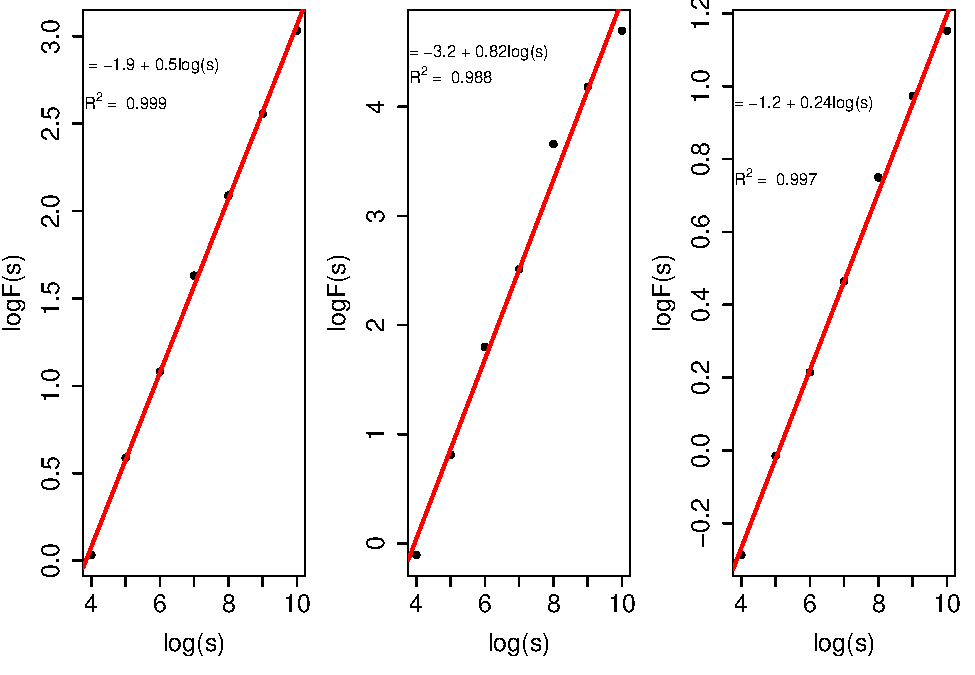
\includegraphics{fractal_regression_paper_brm_files/figure-latex/unnamed-chunk-3-1.pdf}

For an empirical example, we apply the \texttt{dfa()} function to the Human
Balance Dataset (Santos \& Duarte, 2016). This publicly available dataset includes
signals from a force platform measured that measures the center of
pressure in the x and y dimension for 87 young adults (we exclude the
older adults from our analyses for simplicity sake). Trials lasted 60s.
See original paper for additional details on data processing
(Santos \& Duarte, 2016). For the empirical examples, we use two different time
series featuring a participant standing on a firm (rigid) surface with
eyes open and a foam (unstable) surface with eyes open. Note, however,
that we analyze the dataset more fully in INSERT SECTION NAME HERE. We
chose this dataset because postural sway data are known to exhibit
interesting fractal dynamics Delignières, Torre, \& Bernard (2011b) and we can
systematically evaluate the data for all of the univariate and bivariate
analyses detailed in this work.

For center of pressure (COP) data, we take the first order differences
of each series as a rough approximation of COP velocity. For the
univariate analyses, we focus on analyses of the COP data in the x
dimension. Then, we define the appropriate scales for the analyses.

\textbf{Figure 2}

\emph{Log scale-Log fluctuation plots for empirical difference COPx time
series for rigid (left) and unstable (right) surfaces.}

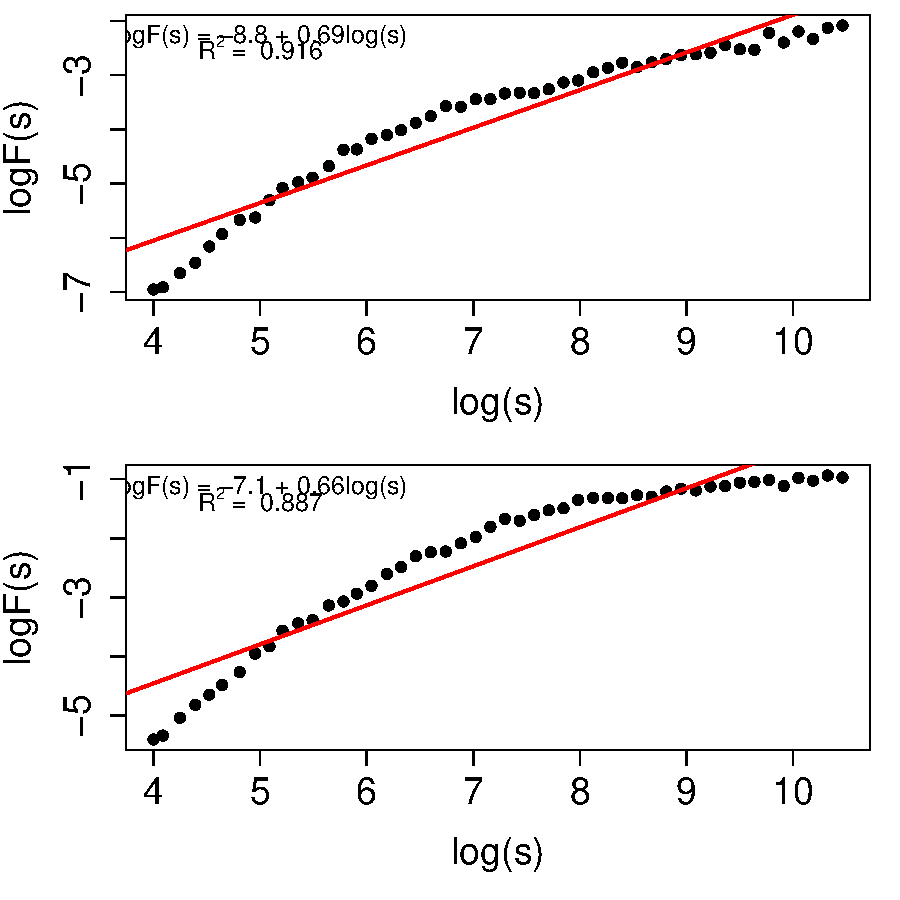
\includegraphics{fractal_regression_paper_brm_files/figure-latex/unnamed-chunk-5-1.pdf}

Importantly, regarding the question one can ask using DFA, we observe
from Figure \#\#, that long range correlations are positive and
approximately 0.69 -
0.66. However, from visual inspection of
these plots we observe that two slopes might fit better than one for
these time series; a phenomenon known as crossovers points Ge \& Leung (2013). One common approach when such crossover points exist is to
recognize that the signal might be best characterized by two scaling
regions, before and after an inflection point. We provide an example of
how to check for where the break point is below using piece-wise
regression.

\begin{verbatim}
## Warning: package 'segmented' was built under R version 4.2.2
\end{verbatim}

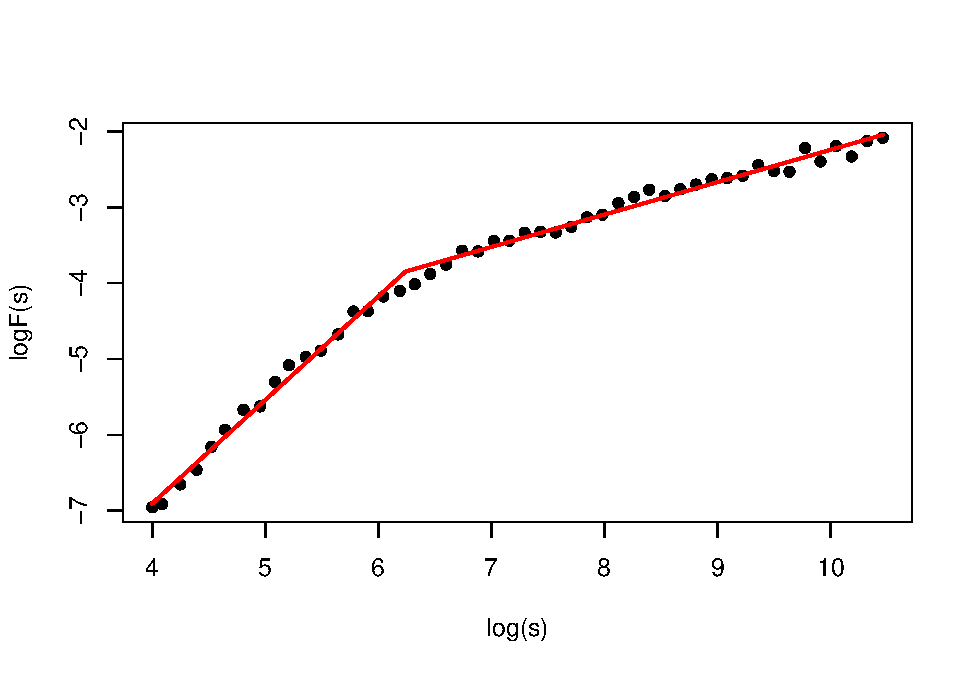
\includegraphics{fractal_regression_paper_brm_files/figure-latex/unnamed-chunk-6-1.pdf}

In the example above, we observe a crossover point at around the scale
size of log 6. And, from the results in Table 2 below, we observe that
there are two distinct scaling relationships corresponding to \(\alpha =\)
1.3 and \(\alpha =\) 0.42, respectively. This is a well known result in
the postural control literature such that short time scales correspond
to persistent temporal correlation and the longer time scales correspond
to anti-persistent correlation. More substantively, short time scale
dynamics correspond to periods of exploratory sway, whereas longer time
scales correspond to corrective movements that prevent exceeding the
base of support and fallingDelignières et al. (2011b).

\textbf{Table 2}

\emph{Results from piece-wise-regression analysis.}

\begin{table}

\centering
\begin{tabular}[t]{l|r|r|r|r|r}
\hline
  & Est. & St.Err. & t value & CI(95\%).l & CI(95\%).u\\
\hline
slope1 & 1.36430 & 0.033533 & 40.686 & 1.29670 & 1.43190\\
\hline
slope2 & 0.42692 & 0.013663 & 31.246 & 0.39938 & 0.45445\\
\hline
\end{tabular}
\end{table}

\hypertarget{multifractal-detrended-fluctuation-analysis}{%
\subsubsection{Multifractal Detrended Fluctuation Analysis}\label{multifractal-detrended-fluctuation-analysis}}

Multifractal Detrended Fluctuation Analysis (MFDFA;
Kantelhardt et al. (2002)) is an extension of DFA
by generalizing the fluctuation function to a range of exponents of the
\(q\)th order. The key question that can be answered by MFDFA is: \emph{how
does the magnitude and direction of long range correlation change over
time within a single time series?} Like DFA, MFDFA entails splitting a
time series into several small bins (e.g., 16). In each bin, least
squares regression is fit and subtracted within each window. However,
the residuals are raised to a range of exponents \(q\) and averaged within
each window. So when \(q = 2\), MFDFA reduces to ordinary DFA. When
\(q >2\), relatively larger residuals are emphasized and when \(q < 2\),
relatively smaller residuals are emphasized. The rest of the DFA
algorithm is performed for each window and windows size for all values
of \(q\). We refer the reader to the work of Kelty-Stephens and colleagues
Kelty-Stephen et al. (2016) Figure 3 for a
visualization of the algorithm and to Kantelhardt and colleagues
Kantelhardt et al. (2002) for additional
mathematical description.

\hypertarget{mfdfa-examples}{%
\subsubsection{MFDFA Examples}\label{mfdfa-examples}}

To demonstrate the use of \texttt{mfdfa()}, we work with data included in our
package (\texttt{fractaldata}), that was originally provided by
E. A. F. Ihlen (2012). It includes a white noise
time series, a monofractal time series, and a multifractal time series.

\textbf{Figure 3}

\emph{Time series from Ihlen (2012) corresponding to white noise,
monofractal, and multifractal series.}

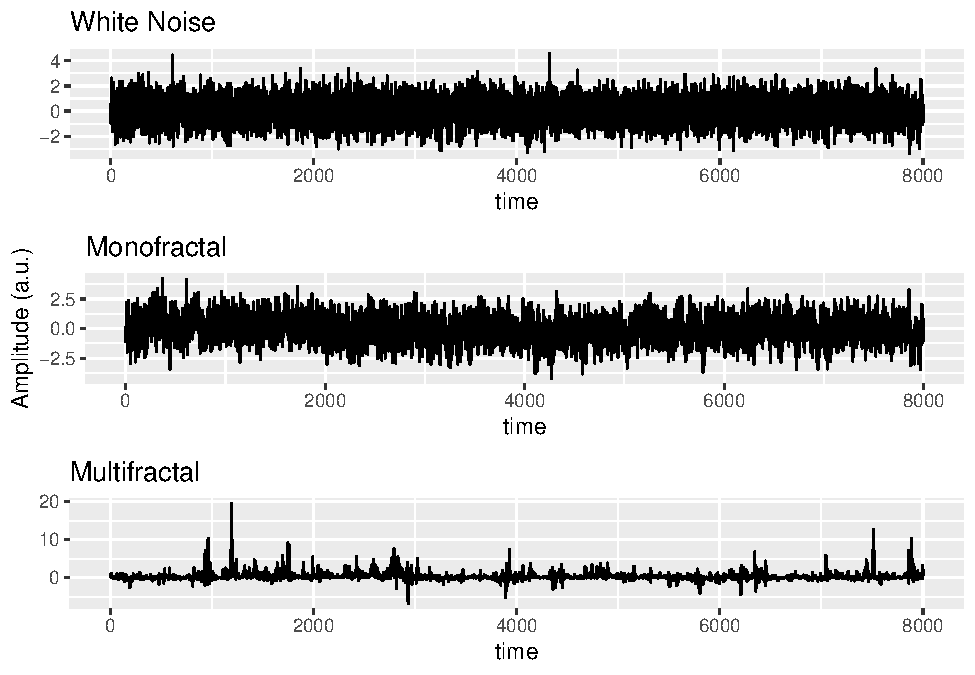
\includegraphics{fractal_regression_paper_brm_files/figure-latex/unnamed-chunk-8-1.pdf}

Performing MFDFA is straight forward with the \texttt{mfdfa()} function. As
shown in the example below, one needs to enter the time series \texttt{x} to
perform the analysis on, the range of \texttt{q} order exponents to use, the
\texttt{order} of polynomial detrending, and the \texttt{scales} for the analysis. In
this case, we define our \texttt{scales} by choosing logarithmically spaced
scales and we select values of q from -5 to 5. Note here that we also
who that the scale factor need not be a power of two but should be
evenly spaced in the logarithmic domain by, for example, using different
logarithm bases. We provide the \texttt{logscale} function to facilitate scale
construction.

\begin{Shaded}
\begin{Highlighting}[]
\NormalTok{scales }\OtherTok{\textless{}{-}} \FunctionTok{logscale}\NormalTok{(}\AttributeTok{scale\_min =} \DecValTok{16}\NormalTok{,}\AttributeTok{scale\_max =} \DecValTok{1024}\NormalTok{,}\AttributeTok{scale\_ratio =} \FloatTok{1.1}\NormalTok{)}

\NormalTok{white.mf.dfa.out }\OtherTok{\textless{}{-}} \FunctionTok{mfdfa}\NormalTok{(}\AttributeTok{x =}\NormalTok{ fractaldata}\SpecialCharTok{$}\NormalTok{whitenoise, }\AttributeTok{q =} \FunctionTok{c}\NormalTok{(}\SpecialCharTok{{-}}\DecValTok{5}\SpecialCharTok{:}\DecValTok{5}\NormalTok{), }\AttributeTok{order =} \DecValTok{1}\NormalTok{, }\AttributeTok{scales=}\NormalTok{scales, }\AttributeTok{scale\_ratio=}\FloatTok{1.1}\NormalTok{)}

\NormalTok{mono.mf.dfa.out }\OtherTok{\textless{}{-}} \FunctionTok{mfdfa}\NormalTok{(}\AttributeTok{x =}\NormalTok{ fractaldata}\SpecialCharTok{$}\NormalTok{monofractal, }\AttributeTok{q =} \FunctionTok{c}\NormalTok{(}\SpecialCharTok{{-}}\DecValTok{5}\SpecialCharTok{:}\DecValTok{5}\NormalTok{), }\AttributeTok{order =} \DecValTok{1}\NormalTok{,  }\AttributeTok{scales=}\NormalTok{scales, }\AttributeTok{scale\_ratio=}\FloatTok{1.1}\NormalTok{)}

\NormalTok{multi.mf.dfa.out }\OtherTok{\textless{}{-}} \FunctionTok{mfdfa}\NormalTok{(}\AttributeTok{x =}\NormalTok{ fractaldata}\SpecialCharTok{$}\NormalTok{multifractal, }\AttributeTok{q =} \FunctionTok{c}\NormalTok{(}\SpecialCharTok{{-}}\DecValTok{5}\SpecialCharTok{:}\DecValTok{5}\NormalTok{), }\AttributeTok{order =} \DecValTok{1}\NormalTok{,  }\AttributeTok{scales=}\NormalTok{scales, }\AttributeTok{scale\_ratio=}\FloatTok{1.1}\NormalTok{)}
\end{Highlighting}
\end{Shaded}

A common way to understand if there is evidence of multifractality is to
examine a plot showing the slopes of the \texttt{log\_fq} at the \texttt{log\_scale}
values. If all the plots have the same slope, that provides evidence of
monofractality. If there are distinct slopes, then there is evidence of
multifractality. It's also important to check here that the slopes of
\texttt{log\_scale} and \texttt{log\_fq} are approximately linear, thus implying that
they are scale invariant. If not, then it could be the case that a
higher order polynomial detrending is appropriate (see Kantelhardt et
al., 2001). Figure 4 shows what we would expect for a monofractal and
multifractal signal. In other words, the monofractal signal shows a
consistent slope, whereas the multifractal signal shows variability in
the slopes.

\textbf{Figure 4}

\emph{mfdfa.plots for mono-(top) and multifractal series (bottom). The four
panels correspond to DETAILS HERE.}

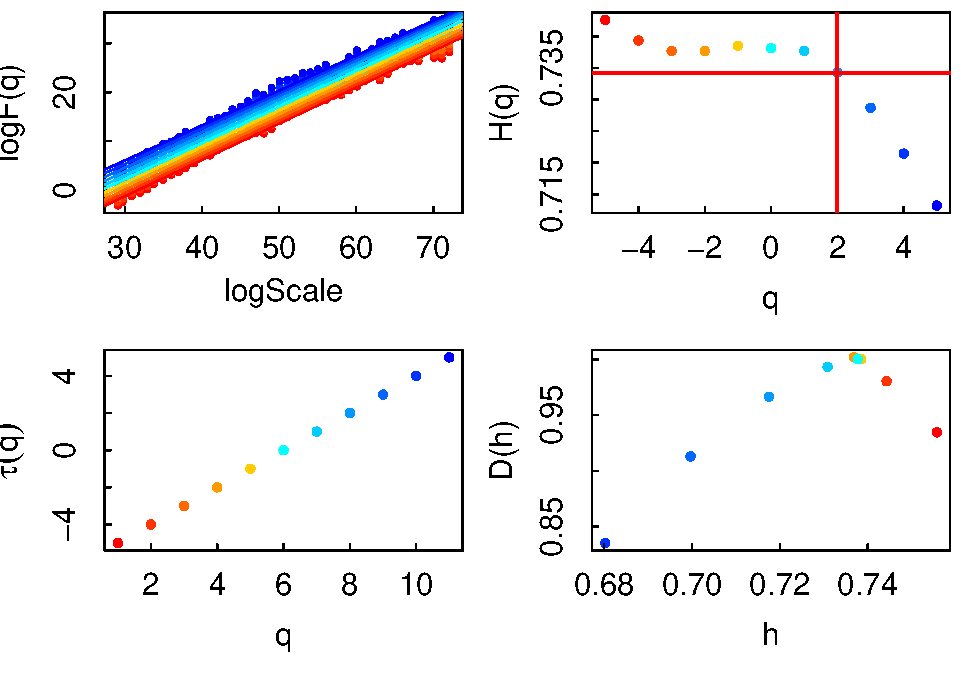
\includegraphics{fractal_regression_paper_brm_files/figure-latex/unnamed-chunk-10-1.pdf} 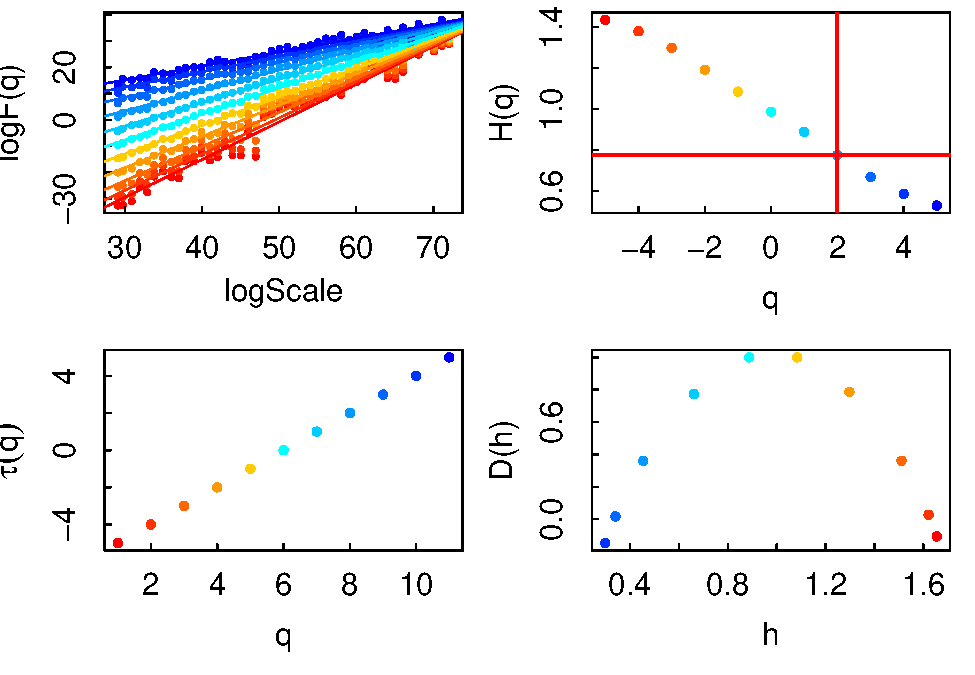
\includegraphics{fractal_regression_paper_brm_files/figure-latex/unnamed-chunk-10-2.pdf}

A common metric for comparing multifractal spectra is to calculate the
width (\(W\)) as \(h_{max} - h_{min}\). Let's do this to compare the
monofractal and multifractal time series. We observe in this case that
for the monofractal signal \(W_{mono} =\)
0.08 and \(W_{multi} =\)
1.36. If plot the
multifractal spectra D(h) against h, we clearly observe the difference
in the widths of the multifractal spectra for the mono- and multifractal
signals, as shown in Figure 4 above.

For our empirical analysis, we again turn to the postural data. We set
out parameters appropriate for the data and run \texttt{mfdfa()}.

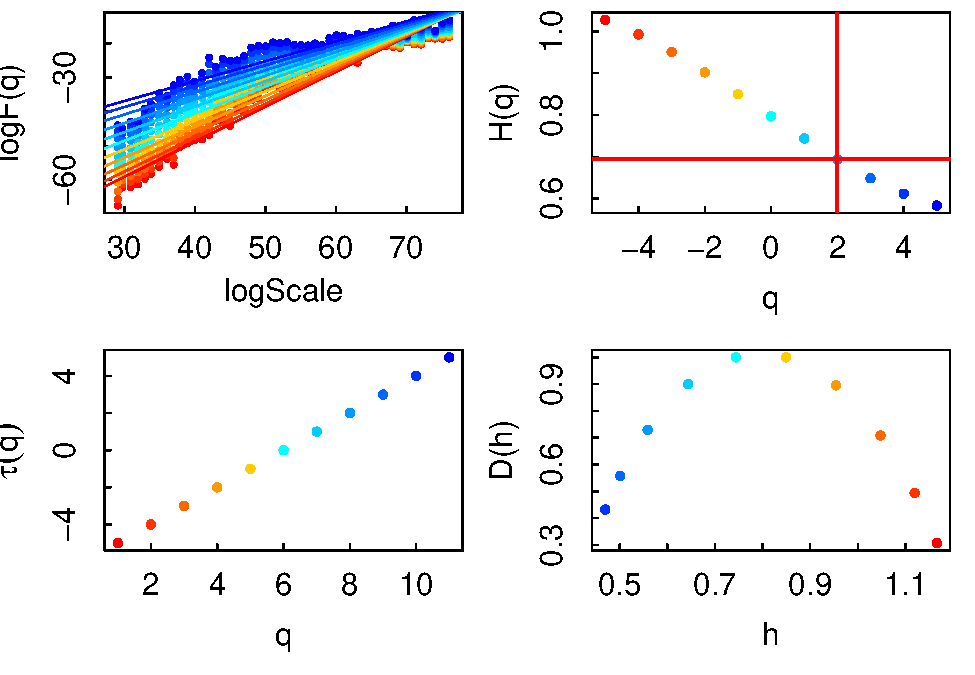
\includegraphics{fractal_regression_paper_brm_files/figure-latex/unnamed-chunk-12-1.pdf} 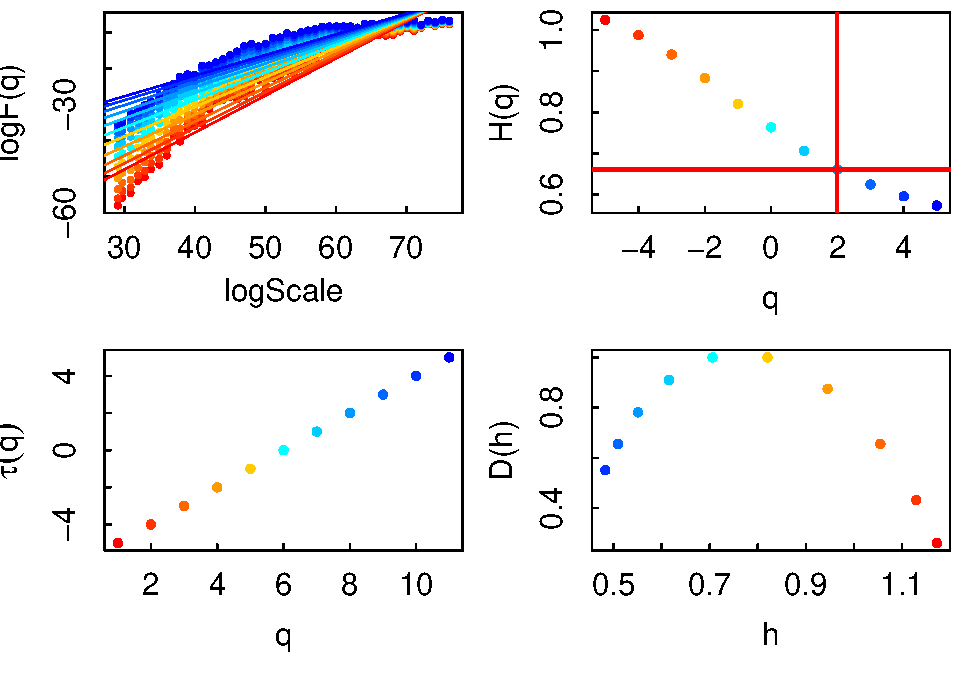
\includegraphics{fractal_regression_paper_brm_files/figure-latex/unnamed-chunk-12-2.pdf}

\hypertarget{dfa-and-mfdfa-considerations}{%
\paragraph{DFA and MFDFA Considerations}\label{dfa-and-mfdfa-considerations}}

We recommend a few points of consideration in using these functions. One
is to be sure to evaluate whether there are cross-over points in the log
scale-log fluctuation plots (Peng et al., 1994; Perakakis, Taylor, Martinez-Nieto, Revithi, \& Vila, 2009). Cross-over points (or a visible change in the slope as
a function of scale) indicate that a simple mono-fractal
characterization does not sufficiently characterize the data. If
cross-over points are evident, we recommend proceeding to estimate the
two scaling regions with a piece-wise regression.

While it is common to use only linear detrending with DFA, this is not
necessarily best practice. Instead, a more rigorous approach requires
inspection trends in the data to determine if a higher order polynomial
would be more appropriate for detrending. One can then compare the DFA
output for different polynomial orders
(Kantelhardt et al., 2001) to determine if a
genuine inflection point is present or if nonlinearity in DFA and MFDFA
emerges due to unadressed nonlinear trends in the original series
(Likens, Amazeen, West, \& Gibbons, 2019b).

General recommendations for choosing the min and max scale are minimum
scale of 10 and a maximum scale of N/4, where N is the total number of
observations in the signal. See Eke et al.~(2002)
(Eke, Herman, Kocsis, \& Kozak, 2002) and Gulich and Zunino (2014)
(Gulich \& Zunino, 2014) for additional considerations
but also keep in mind specific research areas may also have other
criteria Marmelat \& Meidinger (2019).

\hypertarget{bivariate-methods}{%
\subsection{Bivariate Methods}\label{bivariate-methods}}

\hypertarget{detrended-cross-correlation-analysis}{%
\subsubsection{Detrended Cross-Correlation Analysis}\label{detrended-cross-correlation-analysis}}

Detrended Cross-Correlation Analysis (DCCA;
Podobnik and Stanley (2008),
Zebende (2011) ) is a bivariate extension
of the DFA algorithm generalizing it to a correlational case between two
time series that may be non-stationary. The key questions that can be
asked with it are: a) \emph{How does correlation between two time series
change as a function of scale?} and b) \emph{What is/are the dominant (time)
scale(s) of coordination?} Such decisions are based on a predetermined
threshold such as a conventional statistical significance as we
demonstrate below. Researchers may also select other criteria
appropriate for their research area.The DCCA algorithm is a direct
genralization of the DFA algorithm but applied to two concomitantly
measured time series, say \emph{x} and \emph{y}. As in DFA, time series are split
into multiple bins and detrended using least squares regression.
Separate regressions are performed for \emph{x} and \emph{y}. Within each bin,
three quantities are estimated, the average squared residual of \emph{x,} the
average squared residual of \emph{y}, and the average cross product (i.e.,
the covariance) between the residuals for \emph{x} and the residuals for \emph{y}.
Each of those quantities is averaged across all bins of a given size.
After taking the squared residual for \emph{x} and \emph{y}, we obtain scale-wise
equivalents of covariance \(F_{xy}(s)\) and standard deviations for \emph{x}
\(F_x(s)\) and \emph{y} \(F_y(s)\). The use of \(F\) to designate these quantities
derives from originating literatureLikens et al. (2019b). Thus,
the scale-wise regression coefficient, the estimand of DCCA, is nothing
more than the following quotient

\[\rho(s)=\frac{F_{xy}(s)}{F_x(s)F_y(s)}\]

Simplified, with DFA, the key metric is \(\alpha\), but in DCCA, one
estimates the scale-specific, detrended cross-correlation coefficient
\(\rho(s)\) for the pair of time series.

\hypertarget{dcca-examples}{%
\paragraph{DCCA Examples}\label{dcca-examples}}

To demonstrate the use of \texttt{dcca()}, we used the \texttt{mc\_arfima()} function
from our package to simulate two time series with known properties.
Specifically, we use the multicorrelated ARFIMA examples from
Kristoufek's work (Kristoufek, 2013). In
this case, we use the parameters from Kristoufek (2013) for Model 1 (p.
6,487), that generates two time series of length 10,000 that exhibit
long range correlations (LRC) as well as long range cross-correlations
(LRCC). The code for simulating these two time series is shown below.
Additionally, Figure \#, shown below, visualizes a subset of these time
series.

\textbf{Figure \#}

\emph{Subset of two time series exhibiting long range correlation and long
range cross-correlation}

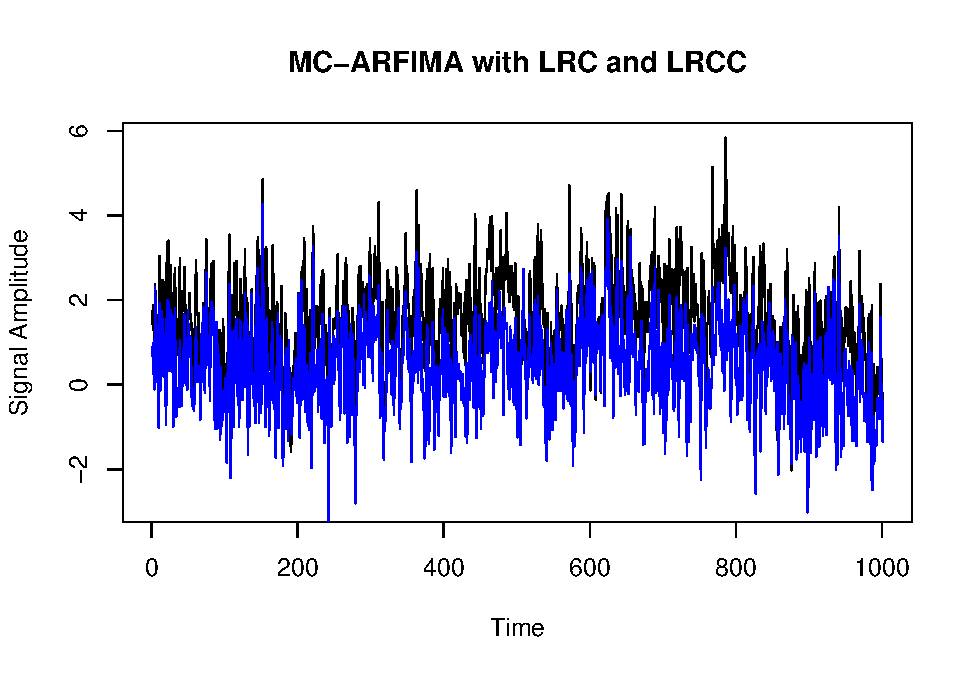
\includegraphics{fractal_regression_paper_brm_files/figure-latex/unnamed-chunk-14-1.pdf}

As can be seen in \hl{Figure **}, the simulated time series, although
quite noisy, appear to covary over time with similar trends. To perform
the \texttt{dcca()} on these time series, we use the code below, where we first
define the \texttt{scales} using the \texttt{logscale()} function described earlier
along with the \texttt{dcca()} function itself.

Next, we visualize the output of DCCA in Figure \#. We observe that, as
expected, the correlation between the MC-ARFIMA processes are
consistently high (all \(\rho\)'s \(> .8\)) and continue to be high at
increasing time scales.

\textbf{Figure \#}

\emph{DCCA output for long range correlation and long range
cross-correlation}

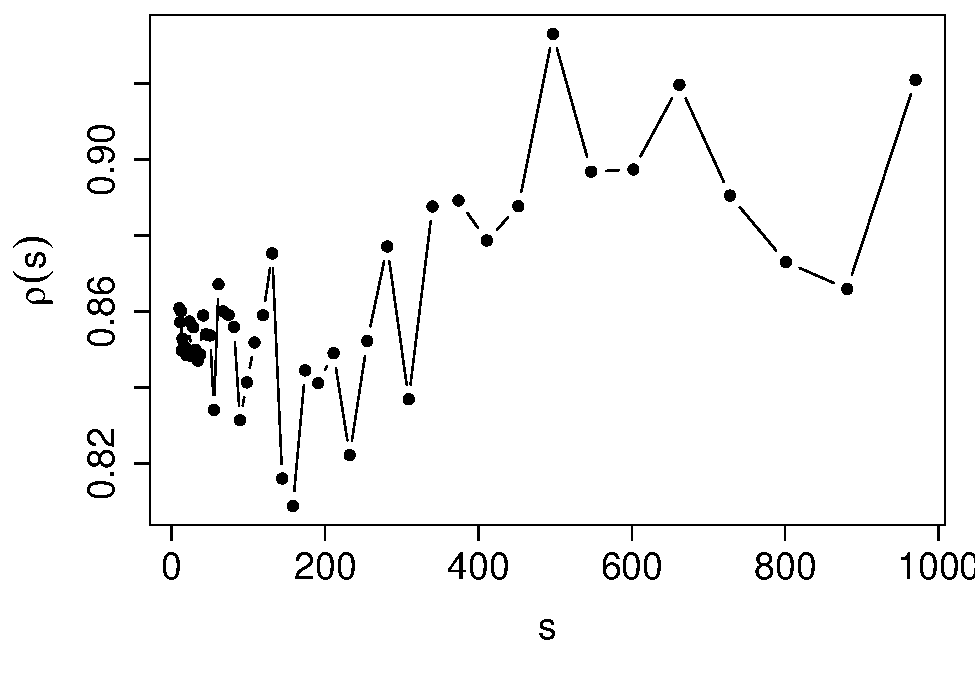
\includegraphics{fractal_regression_paper_brm_files/figure-latex/unnamed-chunk-16-1.pdf}

Figure \#\# is difficult to interpret on its own. Next we demonstrate
additional plot and analysis features of \texttt{dcca()} by modifying the above
code as shown below \texttt{ci\ =\ TRUE}. Loess smoothing can also be applied to
both \(\rho(s)\) and its confidence intervals using \texttt{loess.rho\ =\ TRUE} and
\texttt{loess.ci\ =\ TRUE}. Those latter options are useful for reducing the
impact of increasing variance in estimates of \(\rho(s)\) at large scales
(Likens et al., 2019b). Note though that a much larger set of calculations takes
place and may take sevral seconds up to several minutes (for long time
series) to complete.

\textbf{Figure \#}

\emph{DCCA output for long range correlation and long range
cross-correlation}

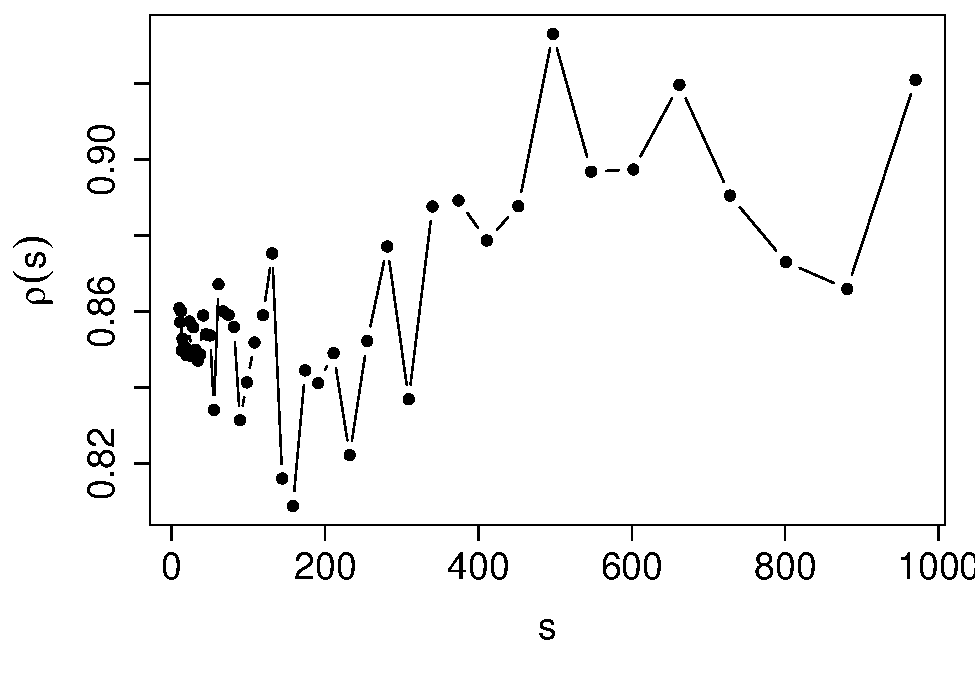
\includegraphics{fractal_regression_paper_brm_files/figure-latex/unnamed-chunk-17-1.pdf}

As a point of comparison, we can generate a time series in contrast with
this that exhibits processes with LRC and short-range cross-correlation
(SRCC) using the code below. In contrast to the previous DCCA analysis,
Figure \# shows a signal that begins with a high cross-correlation
(\(\rho\)'s \(> .6\)) , but that begins to deviate and trend substantially
lower at increasing scale sizes approaching \(\rho = 0\). In fact, based
on the plotted confidence intervals, it is apparent that the correlation
between the two series becomes non-significant from a conventional
statistical standpoint.

\textbf{Figure \#}

\emph{DCCA output for long range correlation and short range
cross-correlation}

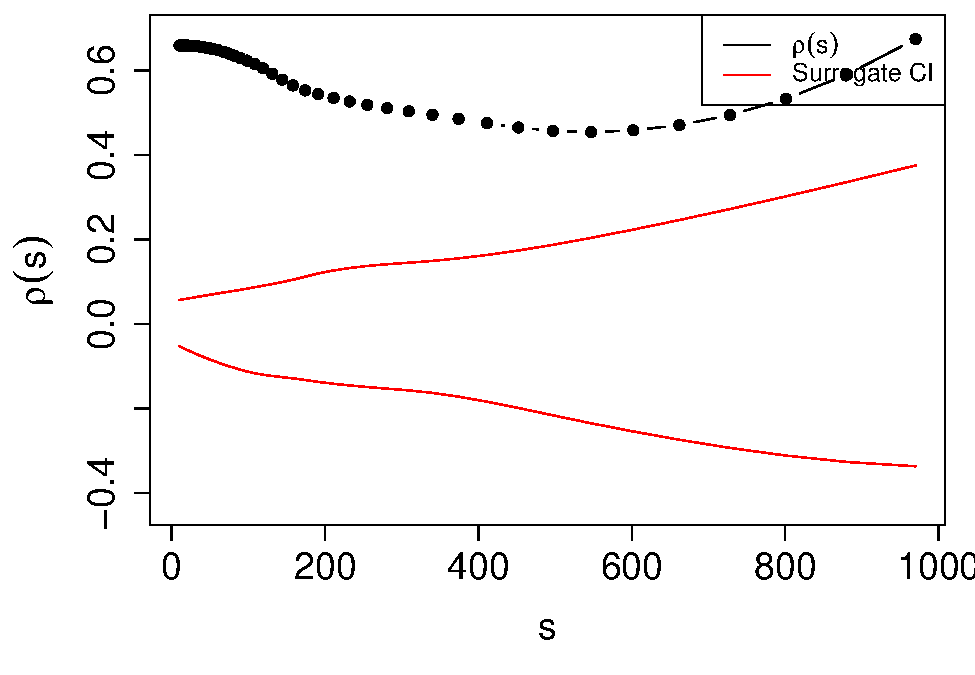
\includegraphics{fractal_regression_paper_brm_files/figure-latex/unnamed-chunk-19-1.pdf}

Turning next to the empirical balance data, we apply DCCA to the
differenced COPx and COPy data for the firm and foam platforms. We again
set appropriate values for \texttt{scales} and apply the \texttt{dcca()} function to
the pairs of time series.

\textbf{Figure \#}

\emph{DCCA output for empirical COPx and COPy balance data for the eyes open
while standing on the firm surface (top) and foam surface (bottom).}

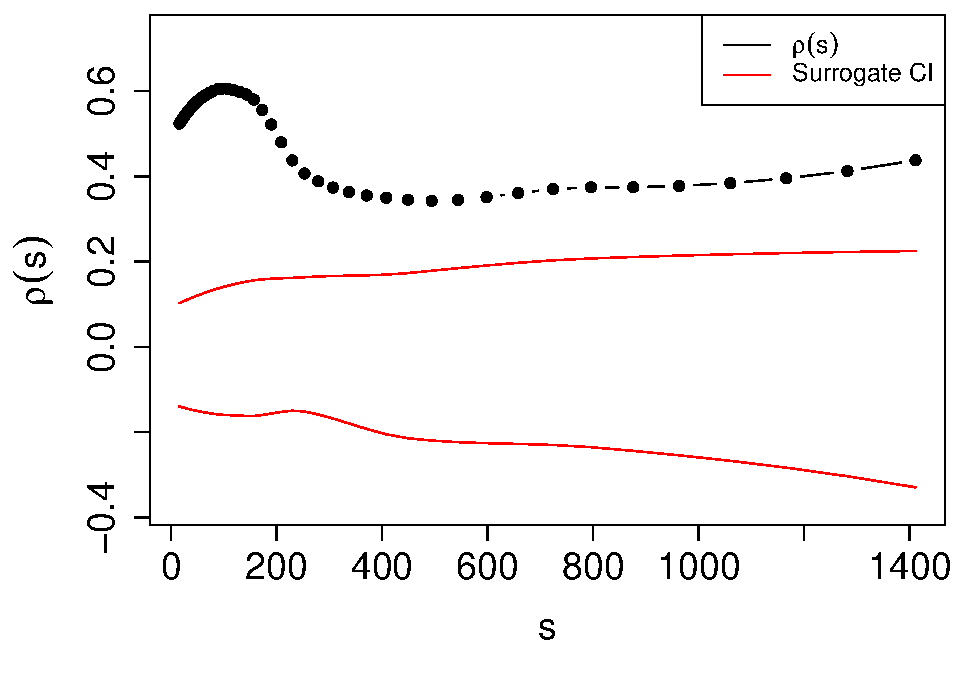
\includegraphics{fractal_regression_paper_brm_files/figure-latex/unnamed-chunk-21-1.pdf} 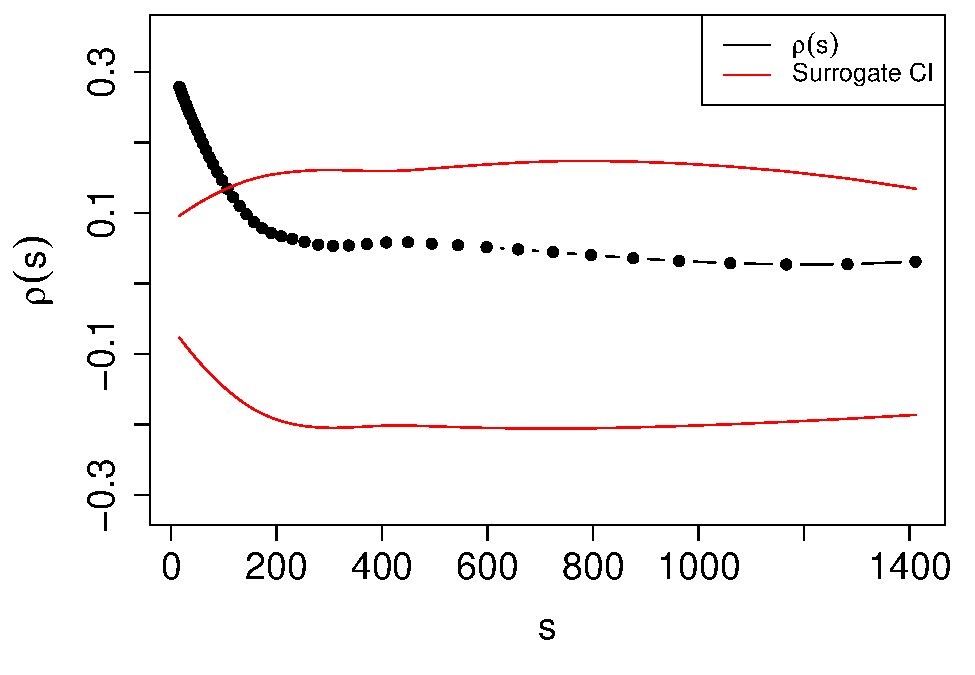
\includegraphics{fractal_regression_paper_brm_files/figure-latex/unnamed-chunk-21-2.pdf}

In examining the output from these analyses, Figure \# shows a clear
difference between the two conditions. First, in the firm platform
example, the \(\rho(s)\) values reach an order of magnitude greater than
in the foam condition with the max \(\rho(s)\) =
0.73' compared to
0.35 for the foam condition. Second, we
observe for the foam example, that the time scale of maximum correlation
is 73,
which is a larger time scale when compared to the foam example, which
had a maximum correlation at scale r
\texttt{dcca.out.open.foam\$scales{[}which.max(dcca.out.open.foam\$rho){]}}. Third,
the pattern of change in correlation across scales is slightly
different. The firm example is higher overall; it starts relatively low
at very small time scales before a rapid increase and then steady
decrease before stabilizing at increasingly larger scales. By contrast,
the foam example has relatively lower overall correlation values, the
smallest scale is the highest followed by a steady decrease and then
also stabilizing at larger scales. Lastly, we can also derive
statistical conclusions because, in the firm condition, the two series
are correlated at all scales, whereas the series are only correlated at
the finest scales in the foam condition.

\hypertarget{multiscale-regression-analysis}{%
\subsubsection{Multiscale Regression Analysis}\label{multiscale-regression-analysis}}

Multiscale regression analysis (MRA) is a further generalization of DCCA
that brings the analyses into a predictive, regression framework
(Kristoufek, 2015b). The key questions that can be answered by it are: a)
\emph{How does the influence of one time series on another time series change
as a function of scale?} and b) \emph{What is/are the dominant (time)
scale(s) of influence of one time series on another time series?} The
algorithm is largely the same as DCCA, with a key difference being that
instead of estimating scale-wise symmetric correlation coefficients,
leveraging methods of Ordinary Least Squares (OLS) regression,
asymmetric \(\beta\) coefficients are estimated (see Likens et al. (2019b);
Kristoufek (2015b) ) according to the following equation

\[
\beta(s)=\frac{F_{xy}(s)}{F^2_x(s)}
\]

The \(\beta(s)\) equation differs from the \(\rho(s)\) equation only in the
denominator where \(F^2_x(s)\) is the average squared residual at each
scale and \(F_xy(s)\) is still the scale-wise covariance.

\hypertarget{mra-examples}{%
\paragraph{MRA Examples}\label{mra-examples}}

Considering the LRC and LRCC simulations used for DCCA, we can examine
whether the scale-wise fluctuations of one variable can predict the
scale-wise fluctuations of the other using \texttt{mra()}. As with a
traditional regression approach, we will use one of our variables as our
predictor (\(x_t\)) and the other as our outcome (\(y_t\)). In the example
below, we again first define our logarithmically spaced scales. We then
apply the \texttt{mra()} function to the two simulated time series. In this
case, it's important to specify which is variable is \texttt{x} (the predictor)
and which is \texttt{y} (the outcome).

We can then visualize these results as shown below in Figure \#.
Generally, we observe that the \(\beta\) coefficients are relatively
stable at increasing time scales with a general, perhaps quadratically
increasing trend. Here it is also important to investigate the change in
\(R^2\) as well as the \(t\)-values. Below we see that the \(R^2\) is quite
high at most of the time scales with \(R^2_{min} =\)
0.67 and \(R^2_{max} =\)
1.85 and all \(\beta(s)\) exceed the confidence
intervals, implying conventional statistical significance. So between
these two component ARFIMA processes, the output of MRA shows that much
of the scale specific variance in \(y_t\) is explained and predicted by
\(x_t\).

\textbf{Figure \#}

\emph{MRA output for long range correlation and long range
cross-correlation.}

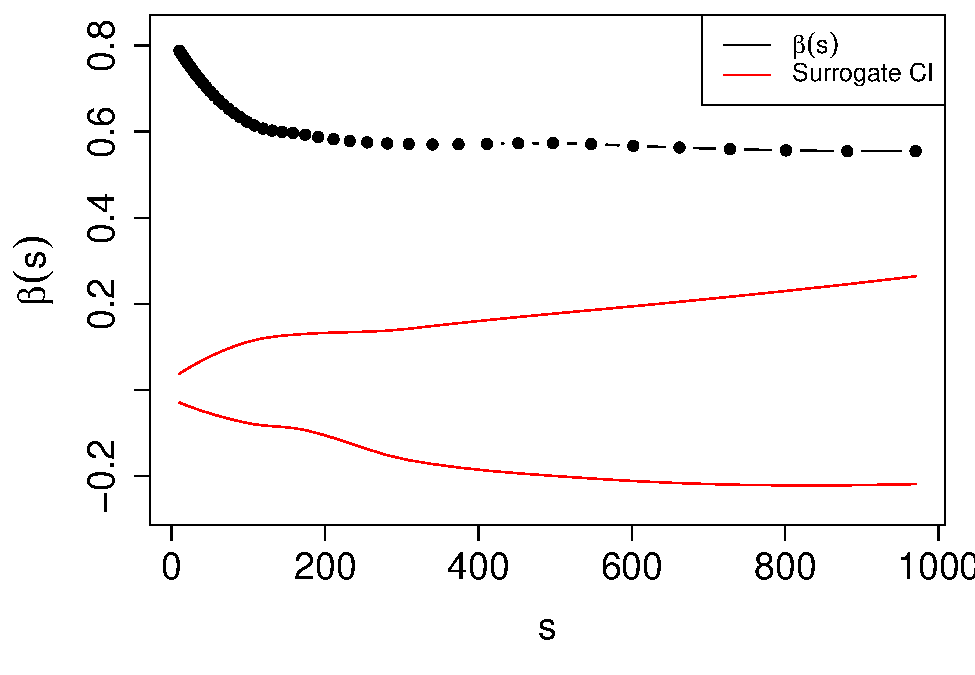
\includegraphics{fractal_regression_paper_brm_files/figure-latex/unnamed-chunk-23-1.pdf}

Turning next to the empirical balance data, we can determine whether
postural adjustments in the COPx are predictive of adjustments in COPy,
and vice versa. This means that we use the \texttt{mra()} function two times
and reverse the order of entry for the x and y arguments to allow for
determining the degree to which each signal can predict the other across
scales. In Figure \# below, we see the resulting \(\beta\)'s we observed
for the the balance data on the firm surface. Notably, the COPx
predicting COPy (max \(\beta\) = 0.19) has
noticeably smaller \(\beta\) values compared to COPy predicting COPx (max
\(\beta\) = 3.25). Notice as well how Figure \#
(bottom), where adjustments in the y dimension are predicting
adjustments in the x dimension, resembles the DCCA plot for this
analysis (see Figure \#). Given the assymetry in the magnitude of the
\(\beta\)s, this example suggests that postural adjustments in the y
dimension appear to be driving changes in the x dimension. And, there is
a clear time scale where this relationship is strongest at scales =
55, implying a
dominant mode of coordination between mediolateral and anterioposterior
control processes.

\textbf{Figure \#}

\emph{MRA output for balance data on foam surface with COPx predicting COPy
(top) and COPy predicting COPx (bottom).}

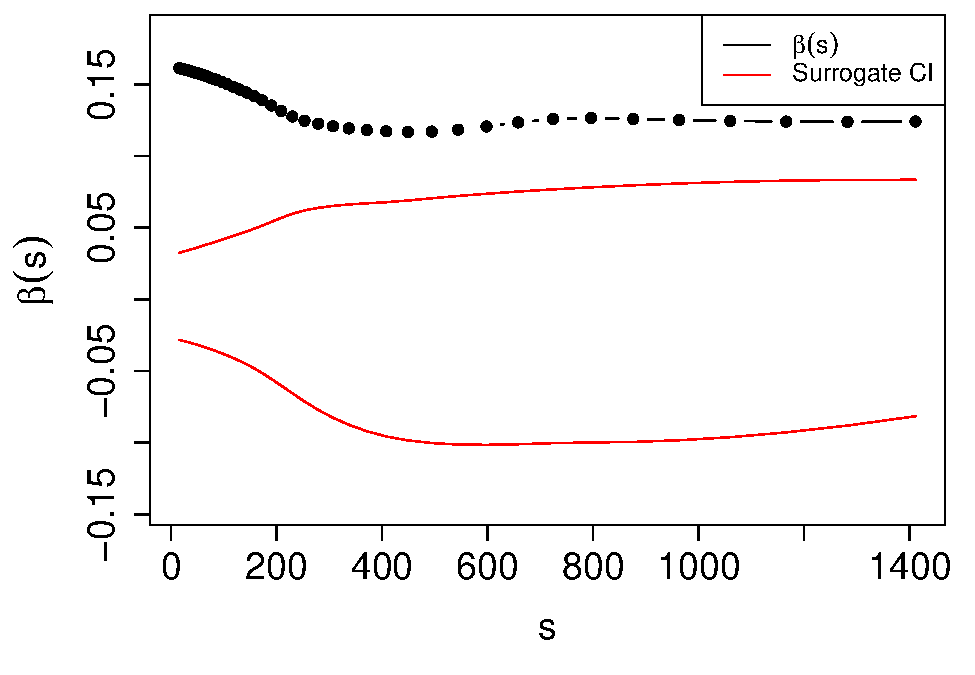
\includegraphics{fractal_regression_paper_brm_files/figure-latex/unnamed-chunk-25-1.pdf} 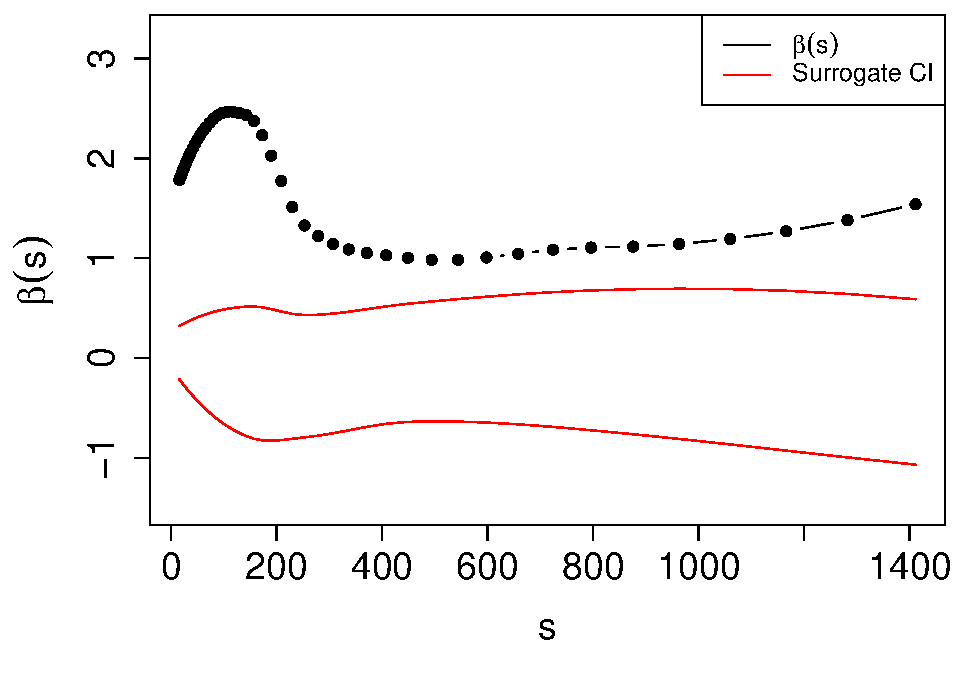
\includegraphics{fractal_regression_paper_brm_files/figure-latex/unnamed-chunk-25-2.pdf}

\hypertarget{multiscale-lagged-regression-analysis}{%
\subsubsection{Multiscale Lagged Regression Analysis}\label{multiscale-lagged-regression-analysis}}

Multiscale lagged regression analysis is an extension of MRA that allows
for examining the influence as a function of scale, but also of time
lag. In particular, the key questions that can be asked with MLRA are:
a) \emph{How does the influence of one time series on another time series
change as a function of scale at different time lags?} and b) \emph{Does the
dominant time scale of influence change over successive time lags?} The
MLRA algorithm performs the same as MRA with a key distinction. It runs
the MRA algorithm for each of a desired number of lags.

\hypertarget{mlra-examples}{%
\paragraph{MLRA Examples}\label{mlra-examples}}

We demonstrate the use of MLRA on a simple two-element system defined
by:

\[
y(t)=1+0.0y(t-50)+1.0x(t-50)+e_1(t)
\]

\[
x(t)=1+0.0y(t-50)+0.0x(t-50)+e_1(t)
\]

In the above system, \(y(t)\) is coupled to \(x(t)\) at lag 50 but \(x(t)\) is
not coupled to \(y(t)\). Running \texttt{mlra()} is the same as \texttt{mra} with one
additional parameter: \texttt{lags}. In Figure \#, we see the output of MLRA
when regressing \(y(t)\) on \(x(t)\) with a maximum lag of 100 time points.
Figure \#\# clearly represents the expected results. There is a strong
positive relationship \(\beta(s,l)\) at lag 50 that clearly approaches
1.0. At other lags however, the values are close to zero.

\textbf{Figure \#}

\emph{MLRA output for simulated simple two-element system regressing} \(y(t)\)
on \(x(t)\)\emph{.}

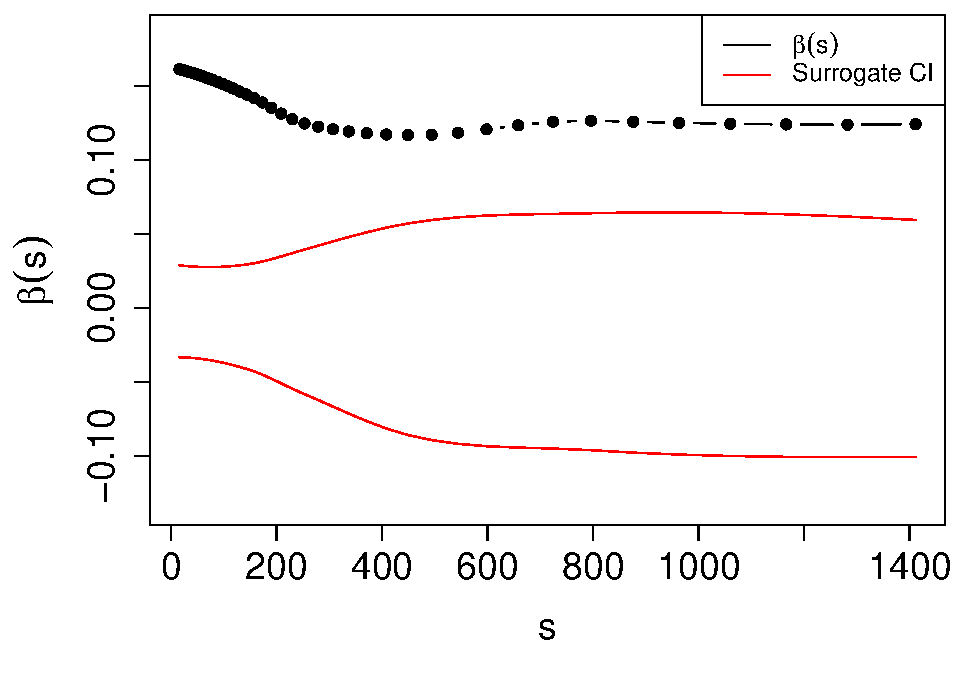
\includegraphics{fractal_regression_paper_brm_files/figure-latex/unnamed-chunk-26-1.pdf}

In terms of the empirical data, below we apply MLRA to the COPxy data
for the firm and the foam examples. Here we also investigate up to a lag
of 100. NEED TO DECIDE ON ORDER HERE FOR MLRA AND ADD SUMMARY OF PLOTS.

\textbf{Figure \#}

\emph{MLRA output for balance data on foam surface with COPx predicting COPy
for the firm (top) and foam (bottom) examples.}

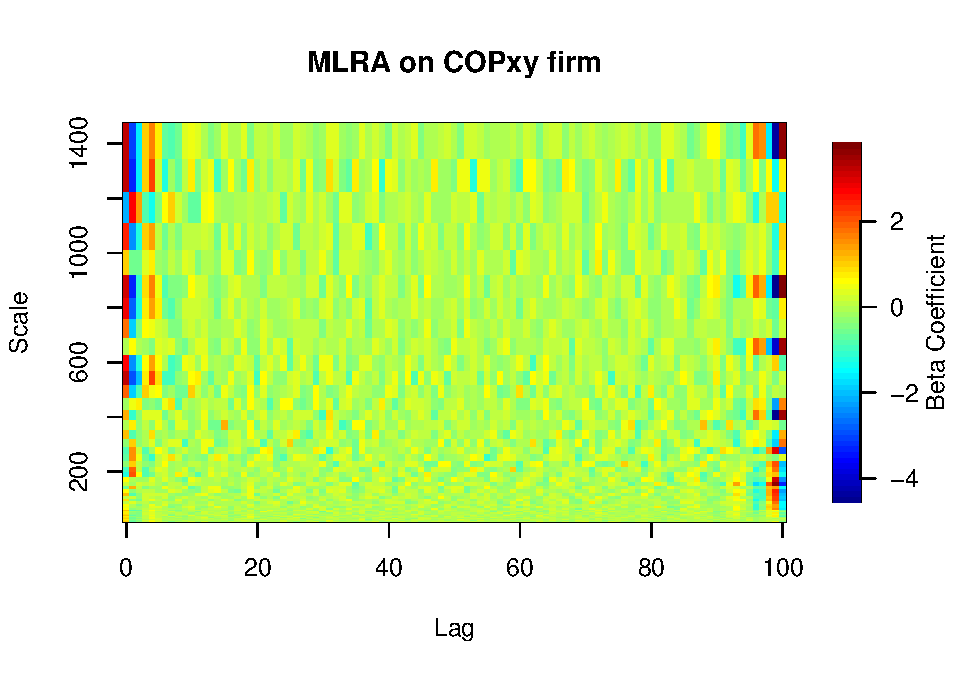
\includegraphics{fractal_regression_paper_brm_files/figure-latex/unnamed-chunk-27-1.pdf} 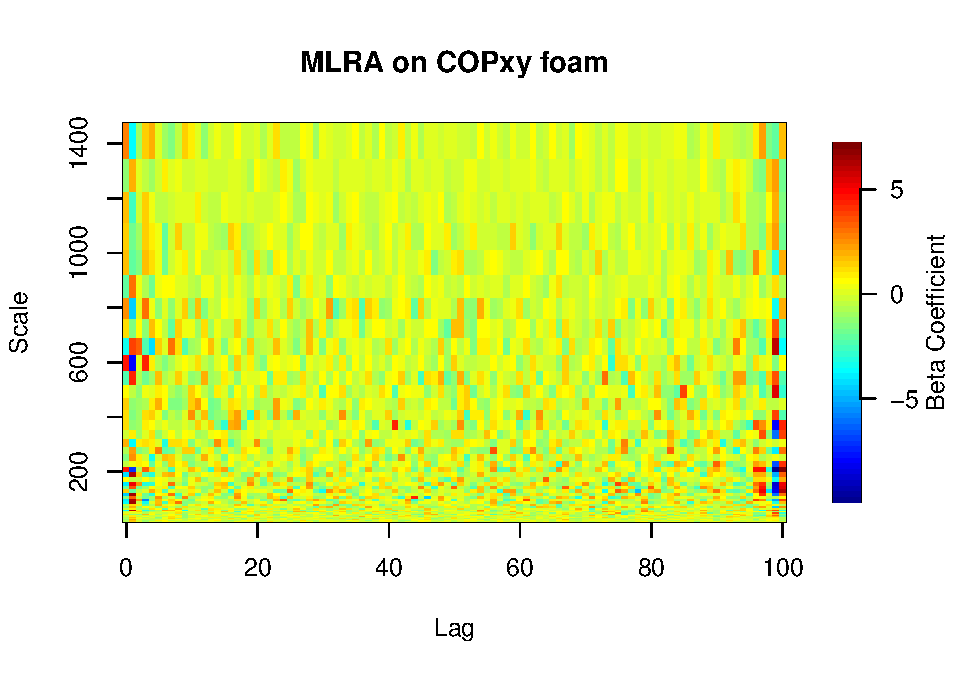
\includegraphics{fractal_regression_paper_brm_files/figure-latex/unnamed-chunk-27-2.pdf}

\hypertarget{surrogate-methods}{%
\subsection{Surrogate Methods}\label{surrogate-methods}}

In all of the above methods, one gets either a single estimate of a
parameter (e.g., \(\alpha\)) or a range of estimates (e.g., \(\rho(s)\),
\(\beta(s)\)). While those estimates are meaningful in and of themselves,
it is common practice to perform some form of null hypothesis test
regarding the estimate(s). These are generally referred to as surrogate
methods Kantz and Schreiber (2003) . We present several options here that could be
ranked in terms of increasing levels of rigor: randomized surrogates,
iterative amplitude adjusted Fourier transformed (IAAFT) surrogates, and
model-based surrogates.

\hypertarget{randomized-surrogates}{%
\subsubsection{Randomized Surrogates}\label{randomized-surrogates}}

Randomized surrogates generally involve randomly shuffling the order of
values of a time series. The idea is generally that the temporal
structure is destroyed, yet the other features of the time series still
exist (Kantelhardt et al., 2002). Note that
additional options exist along these lines (see for example
(Dumas, Nadel, Soussignan, Martinerie, \& Garnero, 2010)). The key comparison here
would be to compare the estimates extracted from a given analysis (e.g.,
DFA) on the observed sample of data with the estimates derived from an
equally sized sample of the surrogate series (see Kantz and Schreiber (2003)
Moulder, Boker, Ramseyer, and Tschacher (2018) (\textbf{wiltshire2019?}) for examples).

Randomizing the pink noise time series, which originally exhibited long
range correlation (\(\alpha\) = 0.82), and performing DFA on
it, now provides an estimate of \(\alpha\) = 0.48,
which is consistent with a random or white noise process. These values
are clearly different, however, performing inferential statistics on a
sample of observed estimates compared to surrogate estimates would
provide compelling evidence that the temporal dynamics suggested by the
observed estimates are different than those derived from a random
process.

\hypertarget{iterative-amplitude-adjusted-fourier-transform-surrogates-iaaft}{%
\subsubsection{Iterative Amplitude-Adjusted Fourier Transform Surrogates (IAAFT)}\label{iterative-amplitude-adjusted-fourier-transform-surrogates-iaaft}}

The IAAFT algorithm was originally developed as a way to discern whether
nonlinearity is a feasible explanation for time series patterns
(Schreiber \& Schmitz, 1996). More recently, it was proposed as a technique to
determine if multifractal indices suggest interaction across scales
(Espen A. F. Ihlen \& Vereijken, 2010). Like with randomized shuffling, estimates derived from
IAAFT surrogates should be also be different from the estimates derived
from the empirical time series. Although in this case, the comparison is
typically made between the multifractal spectra of the observed time
series, and the typical spectrum derived empirically from a set of IAAFT
surrogate series.

In the code below, we provide an example for generating IAAFT surrogates
using the \texttt{iaafft()} function in the package. One enters the \texttt{signal},
which is the observed time series, and \texttt{N}, the number of surrogates to
generate. There are a number of options here but a common number of
surrogates is 19 (Kantz \& Schreiber, 2003), which allows one to establish a 95\%
confidence limit. In practice, surrogates are generated from each
observed time series, but here we illustrate the process using only a
single time series: the multifractal signal used previously in the MFDFA
example. Then we use the same parameters for the \texttt{mfdfa()} function, but
apply it to all of the IAAFFT surrogates. Note also that surrogate
analysis is `built-in' to our plot functions within the package as well
with options to return the relevant empirically derived confidence
intervals.

Assuming we were using IAAFFT to compare the multifractal width (\(W\))
between the observed signal and the surrogate signals, recall that the
observed width was \(W_{multi} =\)
1.36. Now, we can
calculate the average multifractal width across all of the generated
surrogates and we observe that \(W_{surr} =\) 0.60, which is
narrower than the spectrum from the multifractal signal. In practice,
there are many surrogate options (Moulder et al., 2018), but, again, inferential
statistics are commonly performed to compare observed estimates to the
surrogate estimates to bolster evidence of the inferred dynamics.

\hypertarget{model-based-surrogates}{%
\subsubsection{Model-based Surrogates}\label{model-based-surrogates}}

Surrogates can also be generated when a theoretical model exists that
explains the data generating process for the observed time series.
Well-defined mathematical models of this nature are rare in behavioral
sciences, but useful because they allow for more targeted and
(potentially) realistic hypothesis testing of the underlying dynamics
and how they might change due to experimental constraints. We do not
provide a worked out example of such processes, but readers can consult
cited papers for examples of this kind Delignières et al. (2011a).

\hypertarget{general-discussion}{%
\section{General Discussion}\label{general-discussion}}

In this manuscript, we provide details about the first version of a new
R package aimed at bringing together a number of fractal methods that we
and other researchers have found useful in analyzing a range of
behavioral and physiological data. Indeed, these collective methods have
found utility in virtually every area of science. Despite that reach,
many researchers are not aware of these methods or lack software for
their implementation. This \texttt{fractalRegression} package is our effort to
bridge those gaps by demonstrating each of several methods first with
simulated data, followed by equivalent demonstrations with human
movement data. This allows the reader to see both the `best case'
scenario as well as the idiosyncrasies that rear their heads when we
transition from the pristine world of simulation to the noisiness
inherent in human behavioral data.

\begin{itemize}
\item
  General value of methods and the types of questions (mention the
  types of data used in empirical examples.
\item
  Practical consideration of univariate methods

  \begin{itemize}
  \tightlist
  \item
    Length of time series
  \end{itemize}
\item
  Practical consideration of bivariate methods

  \begin{itemize}
  \item
    Length of time series
  \item
    Likens et al.~2019 found positive bias of linear and quadratic
    trends on MRA beta estimates at larger scales that could be
    mitigated with larger detrending order. This involves checking
    the time series with time as a predictor and polynomials.
  \end{itemize}
\item
  Unique contribution of the methods
\item
  Unanswered questions about the methods

  \begin{itemize}
  \item
    When multifractal methods indicate similarity to surrogate for
    some values of q (for example) but not others?
  \item
    Systematic evaluation of simulated data for the bivariate mfdfa
    methods to better understand the methods
  \end{itemize}
\end{itemize}

\hypertarget{appendix-1-fundamental-equations}{%
\section{Appendix 1: Fundamental Equations}\label{appendix-1-fundamental-equations}}

Here we will insert the fundamental equations for showcasing the
algorithms. WE NEED Lagged functions and MFDFA.

DFA

\(F_X = \sqrt{\frac{\sum^{T-s+1}_{j-1}f^2_X(s,j)}{T-s}}\)

where

\(f^2_X(s,j) = \frac{\sum^{j+s-1}_{k=j}(X_k -\widehat{X}_{k,j})}{s-1}\)

DCCA

\(F_Y = \sqrt{\frac{\sum^{T-s+1}_{j-1}f^2_Y(s,j)}{T-s}}\)

where

\(f^2_Y(s,j) = \frac{\sum^{j+s-1}_{k=j}(Y_k -\widehat{Y}_{k,j})}{s-1}\)

and the scale-wise covariance is estimated as:

\(f^2_{XY}(s,j) = \frac{\sum^{j+s-1}_{k=j}(X_k -\widehat{X}_{k,j})(Y_k -\widehat{Y}_{k,j})}{s-1}\)

which forms the basis for the scale-wise correlation coefficient
estimated as:

\(\rho(s) = \frac{F^2_{XY}(s)}{F_X(s)F_Y(s)}\)

and for the multi-scale regression coefficients, we replace the
denominator in the \(\rho(s)\) equation with scale-wise variance of the
predictor to estimate the scale-wise regression coefficient from
regression \(Y_t\) on \(X_t\) as:

\(\widehat{\beta}(s) = \frac{F^2_{XY}(s)}{F^2_X(s)}\)

and where the variance of \(\widehat{\beta}(s)\) is:

\(\sigma_{\widehat{\beta}(s)}^2 = \frac{1}{T-2} \times \frac{F^2_u(s)}{F^2_Y(s)}\)

and the scale-wise residual variance, \(\widehat{F}^2_u(s)\) is estimated
by applying the DFA algorithm to all scale-wise residuals,
\(\widehat{u}_t(s)\) as:

\(\widehat{u}_t(s) = y_t - x_t\widehat{\beta}(s) - \overline{y_t - x_t\widehat{\beta}(s)}\)

\hypertarget{acknowledgments}{%
\section{Acknowledgments}\label{acknowledgments}}

Author AL receives support from a National Institutes of Health Center
grant (P20GM109090), National Science Foundation grant, National
Strategic Research Institute/Department of Defense, and the Nebraska
Collaboration Initiative.

\newpage

\hypertarget{references}{%
\section{References}\label{references}}

\begingroup
\setlength{\parindent}{-0.5in}
\setlength{\leftskip}{0.5in}

\hypertarget{refs}{}
\begin{CSLReferences}{1}{0}
\leavevmode\vadjust pre{\hypertarget{ref-bakSelforganizedCriticalityExplanation1987}{}}%
Bak, P., Tang, C., \& Wiesenfeld, K. (1987). Self-organized criticality: {An} explanation of the 1/f noise. \emph{Physical Review Letters}, \emph{59}(4), 381--384. \url{https://doi.org/10.1103/PhysRevLett.59.381}

\leavevmode\vadjust pre{\hypertarget{ref-bianchi2020}{}}%
Bianchi, S. (2020). Fathon: A python package for a fast computation of detrendend fluctuation analysis and related algorithms. \emph{Journal of Open Source Software}, \emph{5}(45), 1828.

\leavevmode\vadjust pre{\hypertarget{ref-cavanaugh2017}{}}%
Cavanaugh, J. T., Kelty-Stephen, D. G., \& Stergiou, N. (2017). \emph{Multifractality, Interactivity, and the Adaptive Capacity of the Human Movement System: A Perspective for Advancing the Conceptual Basis of Neurologic Physical Therapy}. Retrieved from \url{https://www.ingentaconnect.com/content/wk/npt/2017/00000041/00000004/art00007}

\leavevmode\vadjust pre{\hypertarget{ref-collins1993}{}}%
Collins, J. J., \& De Luca, C. J. (1993). Open-loop and closed-loop control of posture: A random-walk analysis of center-of-pressure trajectories. \emph{Experimental Brain Research}, \emph{95}(2), 308--318. \url{https://doi.org/10.1007/BF00229788}

\leavevmode\vadjust pre{\hypertarget{ref-damouras2010}{}}%
Damouras, S., Chang, M. D., Sejdić, E., \& Chau, T. (2010). An empirical examination of detrended fluctuation analysis for gait data. \emph{Gait \& Posture}, \emph{31}(3), 336--340. \url{https://doi.org/10.1016/j.gaitpost.2009.12.002}

\leavevmode\vadjust pre{\hypertarget{ref-davisMultiscaleInteractionsInterpersonal2016}{}}%
Davis, T. J., Brooks, T. R., \& Dixon, J. A. (2016). Multi-scale interactions in interpersonal coordination. \emph{Journal of Sport and Health Science}, \emph{5}(1), 25--34. \url{https://doi.org/10.1016/j.jshs.2016.01.015}

\leavevmode\vadjust pre{\hypertarget{ref-delignieresMultifractalSignaturesComplexity2016}{}}%
Delignières, D., Almurad, Z. M. H., Roume, C., \& Marmelat, V. (2016). Multifractal signatures of complexity matching. \emph{Experimental Brain Research}, \emph{234}(10), 2773--2785. \url{https://doi.org/10.1007/s00221-016-4679-4}

\leavevmode\vadjust pre{\hypertarget{ref-deligniuxe8res2011}{}}%
Delignières, D., Torre, K., \& Bernard, P. L. (2011a). Interest of velocity variability and maximal velocity for characterizing center-of-pressure fluctuations. \emph{Science \& Motricité}, (74), 31--37. \url{https://doi.org/10.1051/sm/2011107}

\leavevmode\vadjust pre{\hypertarget{ref-delignieresTransitionPersistentAntiPersistent2011}{}}%
Delignières, D., Torre, K., \& Bernard, P.-L. (2011b). Transition from {Persistent} to {Anti}-{Persistent} {Correlations} in {Postural} {Sway} {Indicates} {Velocity}-{Based} {Control}. \emph{PLOS Computational Biology}, \emph{7}(2), e1001089. \url{https://doi.org/10.1371/journal.pcbi.1001089}

\leavevmode\vadjust pre{\hypertarget{ref-delignieresFractalModelsEventbased2008}{}}%
Delignières, D., Torre, K., \& Lemoine, L. (2008). Fractal models for event-based and dynamical timers. \emph{Acta Psychologica}, \emph{127}(2), 382--397. \url{https://doi.org/10.1016/j.actpsy.2007.07.007}

\leavevmode\vadjust pre{\hypertarget{ref-dumasInterBrainSynchronizationSocial2010}{}}%
Dumas, G., Nadel, J., Soussignan, R., Martinerie, J., \& Garnero, L. (2010). Inter-{Brain} {Synchronization} during {Social} {Interaction}. \emph{PLOS ONE}, \emph{5}(8), e12166. \url{https://doi.org/10.1371/journal.pone.0012166}

\leavevmode\vadjust pre{\hypertarget{ref-eddelbuettelRcppSeamlessIntegration2011}{}}%
Eddelbuettel, D., \& Francois, R. (2011). Rcpp: {Seamless} {R} and {C}++ {Integration}. \emph{Journal of Statistical Software}, \emph{40}(1), 1--18. \url{https://doi.org/10.18637/jss.v040.i08}

\leavevmode\vadjust pre{\hypertarget{ref-eddelbuettelRcppArmadilloAcceleratingHighperformance2014}{}}%
Eddelbuettel, D., \& Sanderson, C. (2014). {RcppArmadillo}: {Accelerating} {R} with high-performance {C}++~linear algebra. \emph{Computational Statistics \& Data Analysis}, \emph{71}, 1054--1063. \url{https://doi.org/10.1016/j.csda.2013.02.005}

\leavevmode\vadjust pre{\hypertarget{ref-ekeFractalCharacterizationComplexity2002}{}}%
Eke, A., Herman, P., Kocsis, L., \& Kozak, L. R. (2002). Fractal characterization of complexity in temporal physiological signals. \emph{Physiological Measurement}, \emph{23}(1), R1--R38. \url{https://doi.org/10.1088/0967-3334/23/1/201}

\leavevmode\vadjust pre{\hypertarget{ref-eulerWorkingMemoryPerformance2016}{}}%
Euler, M. J., Wiltshire, T. J., Niermeyer, M. A., \& Butner, J. E. (2016). Working memory performance inversely predicts spontaneous delta and theta-band scaling relations. \emph{Brain Research}, \emph{1637}, 22--33. \url{https://doi.org/10.1016/j.brainres.2016.02.008}

\leavevmode\vadjust pre{\hypertarget{ref-garciaNonlinearTseriesNonlinearTime2020}{}}%
Garcia, C. A. (2020). \emph{{nonlinearTseries}: {Nonlinear} {Time} {Series} {Analysis}}. Retrieved from \url{https://CRAN.R-project.org/package=nonlinearTseries}

\leavevmode\vadjust pre{\hypertarget{ref-ge2013}{}}%
Ge, E., \& Leung, Y. (2013). Detection of crossover time scales in multifractal detrended fluctuation analysis. \emph{Journal of Geographical Systems}, \emph{15}(2), 115--147. \url{https://doi.org/10.1007/s10109-012-0169-9}

\leavevmode\vadjust pre{\hypertarget{ref-goldbergerFractalDynamicsPhysiology2002}{}}%
Goldberger, A. L., Amaral, L. A. N., Hausdorff, J. M., Ivanov, P. C., Peng, C.-K., \& Stanley, H. E. (2002). Fractal dynamics in physiology: {Alterations} with disease and aging. \emph{Proceedings of the National Academy of Sciences}, \emph{99}(suppl 1), 2466--2472. \url{https://doi.org/10.1073/pnas.012579499}

\leavevmode\vadjust pre{\hypertarget{ref-gulichCriterionDeterminationOptimal2014}{}}%
Gulich, D., \& Zunino, L. (2014). A criterion for the determination of optimal scaling ranges in {DFA} and {MF}-{DFA}. \emph{Physica A: Statistical Mechanics and Its Applications}, \emph{397}, 17--30. \url{https://doi.org/10.1016/j.physa.2013.11.029}

\leavevmode\vadjust pre{\hypertarget{ref-hardstoneDetrendedFluctuationAnalysis2012}{}}%
Hardstone, R., Poil, S.-S., Schiavone, G., Jansen, R., Nikulin, V. V., Mansvelder, H. D., \& Linkenkaer-Hansen, K. (2012). Detrended {Fluctuation} {Analysis}: {A} {Scale}-{Free} {View} on {Neuronal} {Oscillations}. \emph{Frontiers in Physiology}, \emph{3}. \url{https://doi.org/10.3389/fphys.2012.00450}

\leavevmode\vadjust pre{\hypertarget{ref-hausdorffFractalDynamicsHuman1996}{}}%
Hausdorff, J. M., Purdon, P. L., Peng, C. K., Ladin, Z., Wei, J. Y., \& Goldberger, A. L. (1996). Fractal dynamics of human gait: Stability of long-range correlations in stride interval fluctuations. \emph{Journal of Applied Physiology}, \emph{80}(5), 1448--1457. \url{https://doi.org/10.1152/jappl.1996.80.5.1448}

\leavevmode\vadjust pre{\hypertarget{ref-ihlenIntroductionMultifractalDetrended2012}{}}%
Ihlen, E. A. F. (2012). Introduction to {Multifractal} {Detrended} {Fluctuation} {Analysis} in {Matlab}. \emph{Frontiers in Physiology}, \emph{3}. \url{https://doi.org/10.3389/fphys.2012.00141}

\leavevmode\vadjust pre{\hypertarget{ref-ihlen2010}{}}%
Ihlen, Espen A. F., \& Vereijken, B. (2010). Interaction-dominant dynamics in human cognition: Beyond 1/{\textflorin}? fluctuation. \emph{Journal of Experimental Psychology: General}, \emph{139}(3), 436--463. \url{https://doi.org/10.1037/a0019098}

\leavevmode\vadjust pre{\hypertarget{ref-kantelhardtDetectingLongrangeCorrelations2001}{}}%
Kantelhardt, J. W., Koscielny-Bunde, E., Rego, H. H. A., Havlin, S., \& Bunde, A. (2001). Detecting long-range correlations with detrended fluctuation analysis. \emph{Physica A: Statistical Mechanics and Its Applications}, \emph{295}(3), 441--454. \url{https://doi.org/10.1016/S0378-4371(01)00144-3}

\leavevmode\vadjust pre{\hypertarget{ref-kantelhardtMultifractalDetrendedFluctuation2002}{}}%
Kantelhardt, J. W., Zschiegner, S. A., Koscielny-Bunde, E., Havlin, S., Bunde, A., \& Stanley, H. E. (2002). Multifractal detrended fluctuation analysis of nonstationary time series. \emph{Physica A: Statistical Mechanics and Its Applications}, \emph{316}(1), 87--114. \url{https://doi.org/10.1016/S0378-4371(02)01383-3}

\leavevmode\vadjust pre{\hypertarget{ref-kantz2003}{}}%
Kantz, H., \& Schreiber, T. (2003). \emph{Nonlinear Time Series Analysis}. Retrieved from \href{https:///core/books/nonlinear-time-series-analysis/519783E4E8A2C3DCD4641E42765309C7}{/core/books/nonlinear-time-series-analysis/519783E4E8A2C3DCD4641E42765309C7}

\leavevmode\vadjust pre{\hypertarget{ref-kelty-stephenThreadingMultifractalSocial2017}{}}%
Kelty-Stephen, D. G. (2017). Threading a multifractal social psychology through within-organism coordination to within-group interactions: {A} tale of coordination in three acts. \emph{Chaos, Solitons \& Fractals}, \emph{104}, 363--370. \url{https://doi.org/10.1016/j.chaos.2017.08.037}

\leavevmode\vadjust pre{\hypertarget{ref-kelty-stephenMultifractalTemporalCorrelations2016}{}}%
Kelty-Stephen, D. G., Stirling, L. A., \& Lipsitz, L. A. (2016). Multifractal temporal correlations in circle-tracing behaviors are associated with the executive function of rule-switching assessed by the {Trail} {Making} {Test}. \emph{Psychological Assessment}, \emph{28}(2), 171--180. \url{https://doi.org/10.1037/pas0000177}

\leavevmode\vadjust pre{\hypertarget{ref-kristoufekMixedcorrelatedARFIMAProcesses2013}{}}%
Kristoufek, L. (2013). Mixed-correlated {ARFIMA} processes for power-law cross-correlations. \emph{Physica A: Statistical Mechanics and Its Applications}, \emph{392}(24), 6484--6493. \url{https://doi.org/10.1016/j.physa.2013.08.041}

\leavevmode\vadjust pre{\hypertarget{ref-kristoufekDetrendedFluctuationAnalysis2015}{}}%
Kristoufek, L. (2015a). Detrended fluctuation analysis as a regression framework: {Estimating} dependence at different scales. \emph{Physical Review E}, \emph{91}(2), 022802. \url{https://doi.org/10.1103/PhysRevE.91.022802}

\leavevmode\vadjust pre{\hypertarget{ref-kristoufek2015}{}}%
Kristoufek, L. (2015b). Detrended fluctuation analysis as a regression framework: Estimating dependence at different scales. \emph{Physical Review E}, \emph{91}(2), 022802. \url{https://doi.org/10.1103/PhysRevE.91.022802}

\leavevmode\vadjust pre{\hypertarget{ref-laibMultifractalAnalysisTime2018}{}}%
Laib, M., Golay, J., Telesca, L., \& Kanevski, M. (2018). Multifractal analysis of the time series of daily means of wind speed in complex regions. \emph{Chaos, Solitons \& Fractals}, \emph{109}, 118--127. \url{https://doi.org/10.1016/j.chaos.2018.02.024}

\leavevmode\vadjust pre{\hypertarget{ref-legrand2003}{}}%
Legrand, P., \& Véhel, J. L. (2003). Signal and image processing with FracLab. \emph{Thinking in Patterns: Fractals and Related Phenomena in Nature}, 321322.

\leavevmode\vadjust pre{\hypertarget{ref-likensStatisticalPropertiesMultiscale2019}{}}%
Likens, A. D., Amazeen, P. G., West, S. G., \& Gibbons, C. T. (2019a). Statistical properties of {Multiscale} {Regression} {Analysis}: {Simulation} and application to human postural control. \emph{Physica A: Statistical Mechanics and Its Applications}, \emph{532}, 121580. \url{https://doi.org/10.1016/j.physa.2019.121580}

\leavevmode\vadjust pre{\hypertarget{ref-likens2019}{}}%
Likens, A. D., Amazeen, P. G., West, S. G., \& Gibbons, C. T. (2019b). Statistical properties of Multiscale Regression Analysis: Simulation and application to human postural control. \emph{Physica A: Statistical Mechanics and Its Applications}, \emph{532}, 121580. \url{https://doi.org/10.1016/j.physa.2019.121580}

\leavevmode\vadjust pre{\hypertarget{ref-likensExperimentalControlScaling2015}{}}%
Likens, A. D., Fine, J. M., Amazeen, E. L., \& Amazeen, P. G. (2015). Experimental control of scaling behavior: What is not fractal? \emph{Experimental Brain Research}, \emph{233}(10), 2813--2821. \url{https://doi.org/10.1007/s00221-015-4351-4}

\leavevmode\vadjust pre{\hypertarget{ref-marmelat2019}{}}%
Marmelat, V., \& Meidinger, R. L. (2019). Fractal analysis of gait in people with parkinson{'}s disease: Three minutes is not enough. \emph{Gait \& Posture}. \url{https://doi.org/10.1016/j.gaitpost.2019.02.023}

\leavevmode\vadjust pre{\hypertarget{ref-moulder2018}{}}%
Moulder, R. G., Boker, S. M., Ramseyer, F., \& Tschacher, W. (2018). Determining synchrony between behavioral time series: An application of surrogate data generation for establishing falsifiable null-hypotheses. \emph{Psychological Methods}, \emph{23}(4), 757--773. \url{https://doi.org/10.1037/met0000172}

\leavevmode\vadjust pre{\hypertarget{ref-pengMosaicOrganizationDNA1994}{}}%
Peng, C.-K., Buldyrev, S. V., Havlin, S., Simons, M., Stanley, H. E., \& Goldberger, A. L. (1994). Mosaic organization of {DNA} nucleotides. \emph{Physical Review E}, \emph{49}(2), 1685--1689. \url{https://doi.org/10.1103/PhysRevE.49.1685}

\leavevmode\vadjust pre{\hypertarget{ref-perakakis2009}{}}%
Perakakis, P., Taylor, M., Martinez-Nieto, E., Revithi, I., \& Vila, J. (2009). Breathing frequency bias in fractal analysis of heart rate variability. \emph{Biological Psychology}, \emph{82}(1), 82--88. \url{https://doi.org/10.1016/j.biopsycho.2009.06.004}

\leavevmode\vadjust pre{\hypertarget{ref-podobnikDetrendedCrossCorrelationAnalysis2008}{}}%
Podobnik, B., \& Stanley, H. E. (2008). Detrended {Cross}-{Correlation} {Analysis}: {A} {New} {Method} for {Analyzing} {Two} {Nonstationary} {Time} {Series}. \emph{Physical Review Letters}, \emph{100}(8), 084102. \url{https://doi.org/10.1103/PhysRevLett.100.084102}

\leavevmode\vadjust pre{\hypertarget{ref-roumeWindowedDetrendedCrosscorrelation2018}{}}%
Roume, C., Almurad, Z. M. H., Scotti, M., Ezzina, S., Blain, H., \& Delignières, D. (2018). Windowed detrended cross-correlation analysis of synchronization processes. \emph{Physica A: Statistical Mechanics and Its Applications}, \emph{503}, 1131--1150. \url{https://doi.org/10.1016/j.physa.2018.08.074}

\leavevmode\vadjust pre{\hypertarget{ref-santos2016}{}}%
Santos, D. A., \& Duarte, M. (2016). A public data set of human balance evaluations. \emph{PeerJ}, \emph{4}, e2648. \url{https://doi.org/10.7717/peerj.2648}

\leavevmode\vadjust pre{\hypertarget{ref-schaworonkowLongitudinalChangesAperiodic2021}{}}%
Schaworonkow, N., \& Voytek, B. (2021). Longitudinal changes in aperiodic and periodic activity in electrophysiological recordings in the first seven months of life. \emph{Developmental Cognitive Neuroscience}, \emph{47}, 100895. \url{https://doi.org/10.1016/j.dcn.2020.100895}

\leavevmode\vadjust pre{\hypertarget{ref-schreiber1996}{}}%
Schreiber, T., \& Schmitz, A. (1996). Improved surrogate data for nonlinearity tests. \emph{Physical Review Letters}, \emph{77}(4), 635--638. \url{https://doi.org/10.1103/PhysRevLett.77.635}

\leavevmode\vadjust pre{\hypertarget{ref-snow2016}{}}%
Snow, E. L., Likens, A. D., Allen, L. K., \& McNamara, D. S. (2016). Taking Control: Stealth Assessment of Deterministic Behaviors Within a Game-Based System. \emph{International Journal of Artificial Intelligence in Education}, \emph{26}(4), 1011--1032. \url{https://doi.org/10.1007/s40593-015-0085-5}

\leavevmode\vadjust pre{\hypertarget{ref-stephenDynamicsInsightMathematical2009}{}}%
Stephen, D. G., Boncoddo, R. A., Magnuson, J. S., \& Dixon, J. A. (2009). The dynamics of insight: {Mathematical} discovery as a phase transition. \emph{Memory \& Cognition}, \emph{37}(8), 1132--1149. \url{https://doi.org/10.3758/MC.37.8.1132}

\leavevmode\vadjust pre{\hypertarget{ref-rcoreteamLanguageEnvironmentStatistical2018}{}}%
Team, R. C. (2018). \emph{R: {A} language and {Environment} for {Statistical} {Computing}}. Vienna, Austria.

\leavevmode\vadjust pre{\hypertarget{ref-vanordenSelforganizationCognitivePerformance2003}{}}%
Van Orden, G. C., Holden, J. G., \& Turvey, M. T. (2003). Self-organization of cognitive performance. \emph{Journal of Experimental Psychology: General}, \emph{132}(3), 331--350. \url{https://doi.org/10.1037/0096-3445.132.3.331}

\leavevmode\vadjust pre{\hypertarget{ref-zebendeDCCACrosscorrelationCoefficient2011}{}}%
Zebende, G. F. (2011). {DCCA} cross-correlation coefficient: {Quantifying} level of cross-correlation. \emph{Physica A: Statistical Mechanics and Its Applications}, \emph{390}(4), 614--618. \url{https://doi.org/10.1016/j.physa.2010.10.022}

\end{CSLReferences}

\endgroup


\end{document}
